%%%%%%%%%%%%%%%%%%%%%%%%%%%%%%%%%%%%%%%%%%%%%%%%%%%%%%%%%%%%%%%%%%%%%%%%%%%%%%%
% File: ornl-template-example.tex
% Authors: Seth R Johnson, *Sam Crawford, and John Batson
% *Corresponding author, crawfordst.@ornl.gov
% Date: Monday April 29 13:41:46 2024
%
% Example of ORNL report template
%%%%%%%%%%%%%%%%%%%%%%%%%%%%%%%%%%%%%%%%%%%%%%%%%%%%%%%%%%%%%%%%%%%%%%%%%%%%%%%
%% Select the appropriate option for a TM [tm], SPR [spr], or LTR [ltr] report.
%\documentclass[tm]{ornltm} % Use for TM report.
%\documentclass[spr]{ornltm} % Use for SPR report.
\documentclass[ltr]{ornltm} % Use for LTR report.

%% Add ``draft'' option to compile more quickly. This option suppresses images links.
%\documentclass[draft,tm]{ornltm} % Use for a TM report in draft mode.


%% Uncomment these to hide a particular page.
%\renewcommand\makeostipage\relax
%\renewcommand\makecoverpage\relax
%\renewcommand\maketitlepage\relax

%% Optional packages that are simply part of this example document
\usepackage{threeparttable} % Table with captions and tablenotes
\usepackage{booktabs} % Toprule, midrule, bottomrule
\usepackage{multirow} % Extend table entries over multiple rows
\usepackage{pdflscape} % Allows landscape pages for wide figures and tables

%% Bibliography styling. WARNING: the biblatex-chicago package removes the
%% footnote rule.
\usepackage[authordate,autocite=inline,backend=biber, natbib]{biblatex-chicago}
%\usepackage{biblatex} % Numerical style

\bibliography{burgers_equation}% Replace with your bib filename.

%% User-specified packages
\usepackage{mathtools}
\usepackage{amsfonts}
\usepackage{setspace}
\usepackage{listings}
\usepackage{subcaption}
\usepackage{pdfpages}
\usepackage{graphicx}
\usepackage{float}
\usepackage{authblk} % Best check on this one...
\usepackage{url}
\usepackage{wrapfig}
\usepackage{physics}
\usepackage[tight]{units}
\usepackage{sectsty}
\usepackage[noabbrev, capitalize]{cleveref}
\usepackage{lipsum}
\usepackage{esint}

\numberwithin{equation}{section}

%% Use inline small italic blue for comments rather than placing them in the
%% margin.
\definecolor{note}{RGB}{48,96,192}
\renewcommand{\marginpar}[1]{{\small\em\color{note}[#1]}}

%%%%%%%%%%%%%%%%%%%%%%%%%%%%%%%%%%%%%%%%%%%%%%%%%%%%%%%%%%%%%%%%%%%%%%%%%%%%%%%
% AUTHORSHIP & PUBLISHING
%%%%%%%%%%%%%%%%%%%%%%%%%%%%%%%%%%%%%%%%%%%%%%%%%%%%%%%%%%%%%%%%%%%%%%%%%%%%%%%

%%% AUTHOR'S LIST
%% Note: multiple authors are separated with the \and command. 
%% Per ORNL guidance, please keep the number of authors at six or fewer.

\author{Liam M. Pohlmann\affilnum{1}}

%%% AUTHOR's LIST WITH AFFILIATIONS (SPR ONLY)
%% Define authors with affiliations. Does not apply to TM or LTR. Comment out if not using.
%% Note: multiple authors are separated with the \and command. 
%% Per ORNL guidance, please keep the number of authors at six or fewer.

%\author{First Author \and Second Author\affilnum{1} \and Third Author\affilnum{2} \and Fourth Author \and Fifth Author \and Sixth Author}

%%% AFFILIATIONS (SPR ONLY)
%% Note: Does not apply to TM or LTR.

\affiliation{%
	\affilnum{1}Oak Ridge National Laboratory \\
	\affilnum{2}University of New Mexico
}

%%% DOCUMENT TITLE
%% Note: if using an explicit line break in the title, you must use the \protect
%% command before it.

\title{Solution of Burgers' Equation Using the Finite Volume Method and Runge-Kutta 4 Time-Stepping Under Various Boundary Conditions}

%%% PUBLICATION DATE
%% Specify date or use current month and year with \today command.

%\date{April 2024}
\date{\today}

%%% REPORT NUMBER
%% Note: This number must match number provided by RESolution.

\reportnum{ORNL/XX-XXXX/XXX} % Replace first XX with TM, SPR, or LTR.

%%% DIVISION NAME
%% Define division/directorate name. Replace ``Division Name'' with your
%% division/directorate.

\division{Nuclear Energy and Fuel Cycle Division}

%%% SPONSOR OPTIONS FOR SPR
%% Leave commented out or remove for TM and LTR.

%%% SPONSOR NUMBER
%% SPR only. Comment out if not using.

%\sponsornum{Sponsor No. (if needed)}

%%% SPONSOR LOGO(s)
%% SPR only. Add sponsor logos by listing file names below. The cover can accommodate two sponsor logos.

%\SponsorLogoOne{luggage/logo-placeholder.jpg} % Sponsor logo one. Comment out if not using.
%\SponsorLogoTwo{luggage/logo-placeholder.jpg} % Sponsor logo two. Comment out if not using.

%%%%%%%%%%%%%%%%%%%%%%%%%%%%%%%%%%%%%%%%%%%%%%%%%%%%%%%%%%%%%%%%%%%%%%%%%%%%%%%
% DOCUMENT RESTRICTIONS
%%%%%%%%%%%%%%%%%%%%%%%%%%%%%%%%%%%%%%%%%%%%%%%%%%%%%%%%%%%%%%%%%%%%%%%%%%%%%%%

%%% DRAFT
%% Mark the report as a draft. Comment out for public release 
%% and unlimited distribution.

\reportdraft

%%% GENERAL RESTRICTIONS
%% Add a restriction notice to the cover page and headers/footers.
%% Select option by removing the % that precedes it.

%\restrict{UT-BATTELLE BUSINESS SENSITIVE}
%\restrict{UT-BATTELLE BUSINESS PERSONAL}
%\restrict{UT-BATTELLE INTERNAL USE ONLY}
%\restrict{Not for public release.}
%\restrict{UNCLASSIFIED CONTROLLED NUCLEAR INFORMATION}

%%% CRADA
%% Add CRADA notice to front cover. Draft or public release are determined
%% by toggling \reportdraft (above).

%\crada{CRADA number NFE-XX-XXXXX}

%%% CUI
%% Add a CUI notice to the header and footer. Use % to toggle on or off. 
%% Note: CUI supercedes restrict. If both are enabled, only CUI will print.
%% Update with appropriate category and designating authority for your document.

%\cui{CUI//CATEGORY/SUBCATEGORY//DISSEM} % Replace with appropriate markings.
%\cuiDA{Authority Name, ORNL} % Define the CUI designating authority. Can be organization, individual, or both.
%\cuiPh{(XXX)~XXX-XXXX} % Define phone number for designated authority.

%%%%%%%%%%%%%%%%%%%%%%%%%%%%%%%%%%%%%%%%%%%%%%%%%%%%%%%%%%%%%%%%%%%%%%%%%%%%%%%


%%%%%%%%%%%%%%%%%%%%%%%%%%%%%%%%%%%%%%%%%%%%%%%%%%%%%%%%%%%%%%%%%%%%%%%%%%%%%%%
% ABBREVIATIONS
%%%%%%%%%%%%%%%%%%%%%%%%%%%%%%%%%%%%%%%%%%%%%%%%%%%%%%%%%%%%%%%%%%%%%%%%%%%%%%%
%% Uses the Acro package called in CLS and styled in the STY. Note that acronyms
%% that aren't used in the document won't be printed in the list.

%\DeclareAcronym{doe}{
%	short = DOE ,
%	long = US Department of Energy
%	 }
%
%\DeclareAcronym{ornl}{
%	short = ORNL ,
%	long = Oak Ridge National Laboratory
%}
%\declareAcronym{cfd}{
%    short=CFD ,
%    long = Computational Fluid Dynamics
%}

%%%%%%%%%%%%%%%%%%%%%%%%%%%%%%%%%%%%%%%%%%%%%%%%%%%%%%%%%%%%%%%%%%%%%%%%%%%%%%%
% FRONT MATTER
%%%%%%%%%%%%%%%%%%%%%%%%%%%%%%%%%%%%%%%%%%%%%%%%%%%%%%%%%%%%%%%%%%%%%%%%%%%%%%%
\begin{document}
	\frontmatter

	\tableofcontents
%% LIST OF FIGURES: optional if fewer than 5 are used
	\listoffigures

%%% LIST OF TABLES: optional if fewer than 5 are used
%\listoftables
%
%%% Print LIST OF ABBREVIATIONS (optional)
%\printacronyms


%%%%%%%%%%%%%%%%%%%%%%%%%%%%%%
%%% ADDITIONAL FRONT MATTER (OPTIONAL)
	\section*{Foreword}
	This research was supported in part by an appointment to the Oak Ridge National Laboratory Research Student Internships Program, sponsored by the US Department of Energy and administered by the Oak Ridge Institute for Science and Education.
	The author would also like to thank Drs. Vineet Kumar, Vivek Rao, and Arpan Sircar for their support of this project through its lifetime.


%%%%%%%%%%%%%%%%%%%%%%%%%%%%%%%%%%%%%%%%%%%%%%%%%%%%%%%%%%%%%%%%%%%%%%%%%%%%%%%
% ABSTRACT
%%%%%%%%%%%%%%%%%%%%%%%%%%%%%%%%%%%%%%%%%%%%%%%%%%%%%%%%%%%%%%%%%%%%%%%%%%%%%%%
	\mainmatter
%\begin{abstract}
%
%The abstract, if short, is inserted here (after \verb|\mainmatter|) before the
%introduction section. If the abstract is long, then it should be inserted
%\emph{before} \verb|\mainmatter|, and the introduction below will be the first
%entry on the page. This \acl{tm} class is used for reports at \acl{ornl}.
%
%\end{abstract}

%%%%%%%%%%%%%%%%%%%%%%%%%%%%%%%%%%%%%%%%%%%%%%%%%%%%%%%%%%%%%%%%%%%%%%%%%%%%%%%
% DOCUMENT CONTENT
%%%%%%%%%%%%%%%%%%%%%%%%%%%%%%%%%%%%%%%%%%%%%%%%%%%%%%%%%%%%%%%%%%%%%%%%%%%%%%%
	\acresetall % Reset abbreviations for narrative.


	\section{Problem Statement} \label{sec:problem-statement}
	Burgers' equation is a 1D partial differential equation (PDE) developed as a model to understand fluid flow.
	This equation specifically enables the exploration of shocks and rarefactions in fluids, which are discontinuous solutions.
	It is given as~\autocite{salihBurgersEquation2016}:
	\begin{equation}
		\label{eq:burgers-equation}
		\pdv{u}{t} + u\pdv{u}{x} = \nu \pdv[2]{u}{x}
	\end{equation}
	or, using different notation:
	\begin{equation}
		\label{eq:alternate-burgers-equation}
		u_t + uu_x=\nu u_{xx}
	\end{equation}
	\Cref{eq:burgers-equation}'s terms are physically understood as:
	\begin{equation*}
		\begin{split}
			\pdv{u}{t}&=\text{Time-dependent term}\\
			u\pdv{u}{x}&=\text{Advection term}\\
			\nu \pdv[2]{u}{x}&=\text{Diffusion term}
		\end{split}
	\end{equation*}
	For this paper, we choose the initial conditions to be a piecewise-defined step function:
	\begin{equation}
		\label{eq:initial-condition}
		u(x,0)=\begin{cases}
				   u_L, & x<L/2\\
				   u_R, & x\geq L/2
		\end{cases}
	\end{equation}
	in the domain $x\in [0,L]$, $t\in[0,T]$.
	To close the system, the following three boundary conditions will be considered:
	\begin{enumerate}
		\item Inhomogeneous Dirichlet
		\item Inhomogeneous Neumann
		\item Periodic
	\end{enumerate}
	These are discussed in further detail in \cref{subsec:dirichlet,subsec:neumann,subsec:periodic}.


	\section{Finite Volume Method}\label{sec:finite-volume-method}
	In the finite volume method (FVM), the spatial domain is discretized into a set of volumes.\footnote{In 1D, the ``volumes'' are simply line segments.}
In the FVM, unlike the finite element method, information is stored at the center of the volume.
The goal has thus been changed from solving directly for $u$ and now for $\bar{u}$, which is defined as:
\begin{equation}
	\label{eq:u-bar}
	\begin{split}
		\bar{u}&=\frac{\int_{\Omega_V} u \dd \Omega_V }{\int_{\Omega_V}\dd \Omega_V }\\
		&=\frac{1}{V}\int_{\Omega_V} u \dd \Omega_V
	\end{split}
\end{equation}
where $\Omega_V$ defines the spatial domain of a single arbitrary volume in the global domain, $\Omega$.
\Cref{fig:domain and subdomain} provides a graphical representation.
The second line in \cref{eq:u-bar} defines $V\equiv\int_{\Omega_V}\dd \Omega_V $, the cell volume, and simplifies the first line.
Notice that \cref{eq:u-bar} defines the \textit{volume-averaged} value of $u$ in the cell.
The implicit assumption is that $u$ varies only slightly in the volume, and this assumption is valid with a sufficiently small spatial discretization.
\begin{figure}
	\centering
	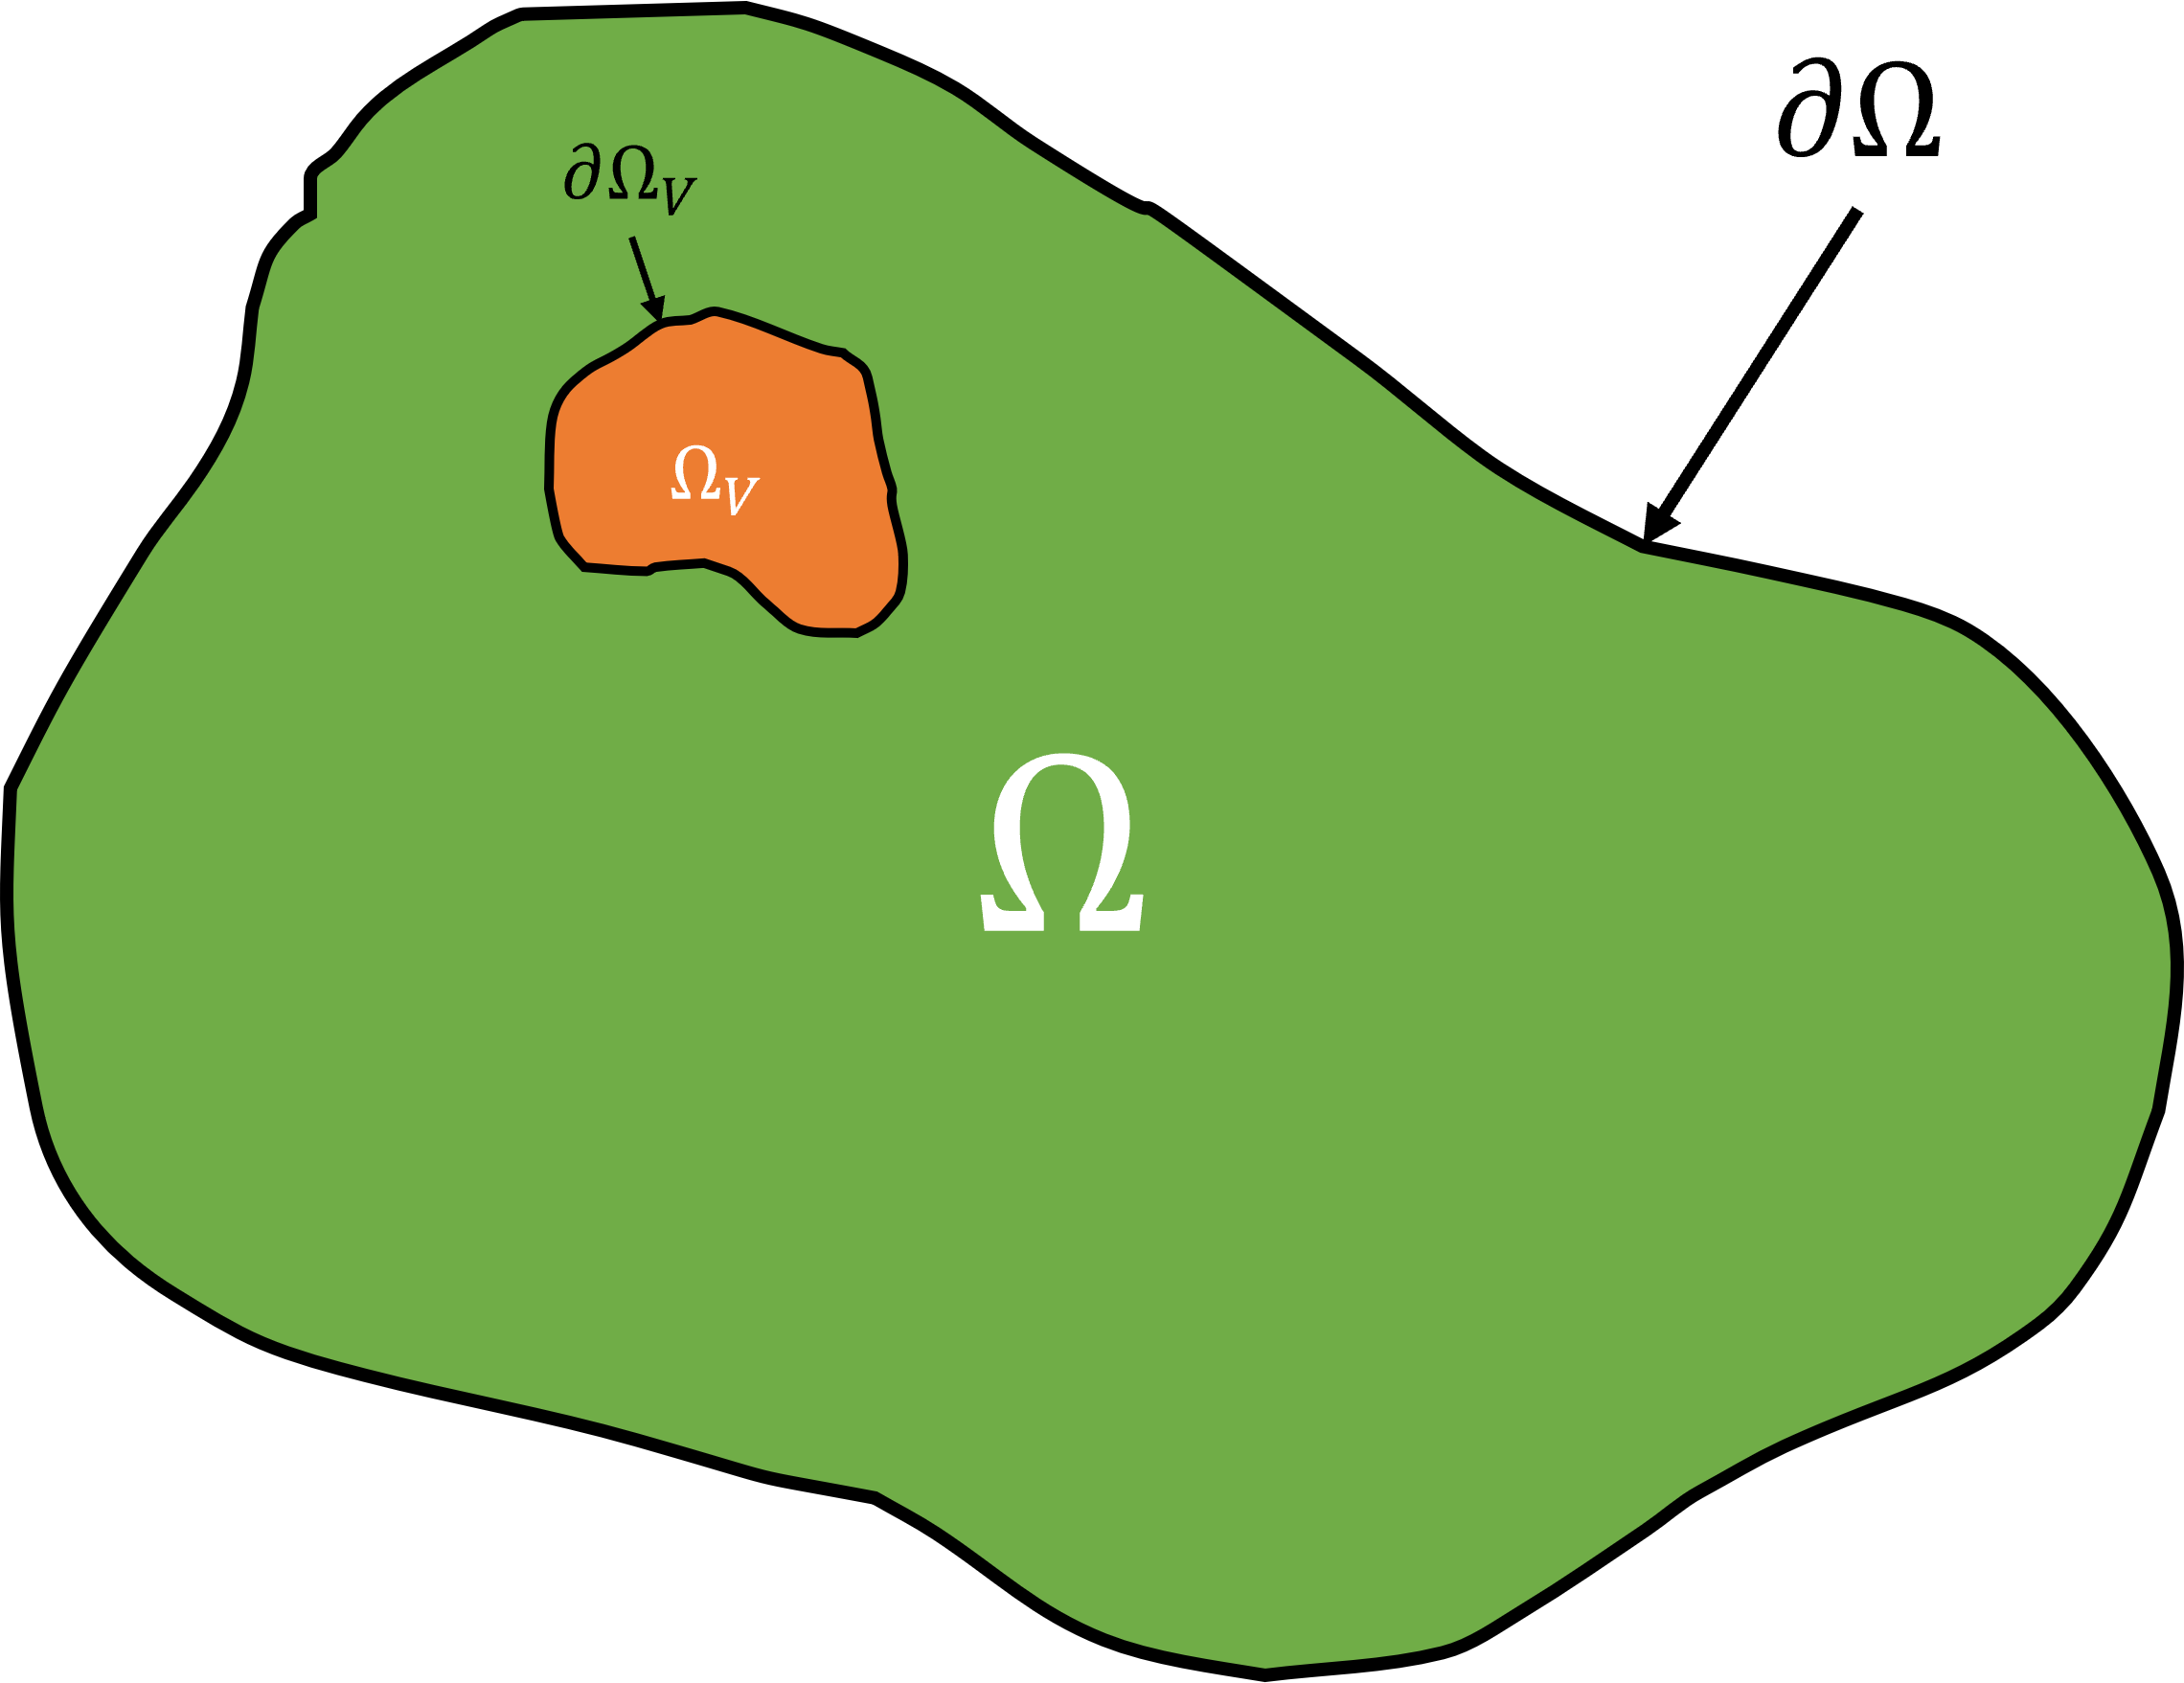
\includegraphics[width=0.6\textwidth]{figures/domain_subdomain}
	\caption{Arbitrary domain and volume subdomain.}
	\label{fig:domain and subdomain}
\end{figure}
Substituting \cref{eq:u-bar} into \cref{eq:burgers-equation} gives the following:
\begin{equation}
	\label{eq:u-averaged-burgers}
	\pdv{\bar{u}}{t} + \bar{u}\pdv{\bar{u}}{x} = \nu \pdv[2]{\bar{u}}{x}
\end{equation}

\Cref{eq:u-bar} has only integrated the function over a discretized volume, not the entire domain, giving the average value of the function within the volume.
Integrating over the entire spatial domain gives\footnote{This is the main step of the FVM, and it carries with it important properties of conservation. Therefore, for applications such as fluid mechanics, properties such as mass are guaranteed to be conserved, leading to a physically-representative solution.}:
\begin{equation}
	\label{eq:finite-volume-aribitrary-domain}
	\int_{\Omega}\bar{u}_t \dd \Omega + \int_{\Omega}  \bar{u}\bar{u}_x\dd \Omega = \int_{\Omega}\nu \bar{u}_{xx}\dd \Omega
\end{equation}
\Cref{eq:finite-volume-aribitrary-domain} was written with a more general notation where $\Omega$ is some arbitrary domain.
When the domain is in 1D and has been discretized into $m$ finite volumes, the system would instead be written as:
\begin{equation}
	\label{eq:finite-volume-implemented}
	\sum_{i=0}^{m-1} \left[  \int_{i-1/2}^{i+1/2} \bar{u}_t \dd \left(\Omega_V\right)_i+\int_{i-1/2}^{i+1/2} \bar{u}\bar{u}_x \dd \left(\Omega_V\right)_i \right]=\sum_{i=0}^{m-1}\left[ \int_{i-1/2}^{i+1/2} \nu \bar{u}_{xx}\dd \left(\Omega_V\right)_i \right]
\end{equation}
The index $i$ represents the center of the volume, so $i\pm 1/2$ is boundary of the volume.
Applying the divergence theorem\footnote{This step may seem overcomplicated, but it is ubiquitous in FVM methods, particularly for more complicated equations such as the Navier-Stokes. This step is introduced this way to ensure the reader understands its importance, trivial as it may be for a 1D case.}, which is defined as~\autocite{CalculusIIIDivergence}:
\begin{equation}
	\label{eq:divergence-thm}
	\iiint_{\Omega}\div \vec{f}\dd V = \oiint_{\partial \Omega} \vec{f}\cdot \hat{n}\dd S
\end{equation}
where $\vec{f}$ is some vector-valued function, $\Omega$ is an arbitrary domain, and $\partial \Omega$ is the domain's boundary, gives the following:
\begin{equation}
	\label{eq:finite-volume-solution}
	\bar{u}_t \Delta x +\left( \left( \frac{\bar{u}^2}{2}\right)_{i+1/2}-\left( \frac{\bar{u}^2}{2}\right)_{i-1/2} \right)=\nu \left( \pdv{\bar{u}}{x}\eval_{i+1/2}-\pdv{\bar{u}}{x}\eval_{i-1/2} \right)
\end{equation}
It is noted that a shortcut has been taken in the first integral:
\begin{equation*}
	\begin{split}
		\int_{i-1/2}^{i+1/2} \bar{u}_t \dd \left(\Omega_V\right)_i&=\bar{u}_t\int_{i-1/2}^{i+1/2} \dd \left(\Omega_V\right)_i\\
		&=\bar{u}_{t}V_i
	\end{split}
\end{equation*}
where $V_i$ is the volume of $i$\textsuperscript{th} volume.
$V_i$ in 1D is simply the length along the domain.
More on this is discussed in \cref{sec:boundary-conditions-and-implementation}, but for now, assume the domain has been discretized into equally-spaced, 1D volumes of length $\Delta x$.

Herein lies a conundrum.
To solve \cref{eq:finite-volume-solution}, both the functional values and the derivatives at the boundaries must be known.
As discussed with \cref{eq:u-bar}, only the average value of the cell is known.
Necessarily, the solution is assumed and often expected to be discontinuous on the volume boundaries.\footnote{A perfectly continuous case would imply a steady solution with no spatial variation.}

Approximation techniques are now used to describe these values.
The derivatives at the boundaries can be approximated in a straightforward manner with finite differencing.
To derive the stencil, one expands $\pdv{u}{x}\eval_{i\pm 1/2}=u_x\eval_{i\pm 1/2}$ using two Taylor series~\autocite{yewNumericalDifferentiationFinite2011a}:
\begin{subequations}
	\begin{equation}
		\label{eq:first-taylor-expansion}
		u_x\eval_{i+1/2}=u_x\eval_i+\left( \frac{\Delta x}{2} \right)u_{xx}\eval_{i}+\frac{1}{2!}\left( \frac{\Delta x}{2} \right)^2 u_{xxx}\eval_i+\order{\left( {\Delta x} \right)^3}
	\end{equation}
	\begin{equation}
		\label{eq:second-taylor-expansion}
		u_x\eval_{i-1/2}=u_x\eval_i-\left( \frac{\Delta x}{2} \right)u_{xx}\eval_{i}+\frac{1}{2!}\left( \frac{\Delta x}{2} \right)^2 u_{xxx}\eval_i+\order{\left( {\Delta x} \right)^3}
	\end{equation}
\end{subequations}
The subscript $x$ in $u_x$ indicates a derivative with respect to $x$, so $u_{xx}=\pdv[2]{u}{x}$ and $u_{xxx}=\pdv[3]{u}{x}$.
The symbol $\order{}$ is known as ``big-O'' notation, and it describes the dominant term in an infinite series.
Because $\left( \Delta x \right)^3>\left( \Delta x \right)^4>\ldots$, it is said that the error terms increase on an ``order of $\left( \Delta x \right)^3$.''
Subtracting \cref{eq:second-taylor-expansion} from \cref{eq:first-taylor-expansion} gives the following:
\begin{equation}
	\label{eq:flux-difference-result}
	u_x\eval_{i+1/2}-u_x\eval_{i-1/2}=\Delta x u_{xx}\eval_i+\order{ (\Delta x)^3 }
\end{equation}
An approximation for $u_{xx}\eval_i$ must now be found.
Fortunately, this process is simple because resources such as~\autocite{yewNumericalDifferentiationFinite2011a} have already derived high-order methods, such as two-point central differencing, for finding the value of the derivative at a volume center.
\begin{equation}
	\label{eq:spatial-finite-difference-2nd-derivative}
	u_{xx}\eval_i=\frac{u_{i+1}-2u_i+u_{i-1}}{\left( \Delta x \right)^2}+\order{\left(\Delta x \right)^2}
\end{equation}
\Cref{eq:spatial-finite-difference-2nd-derivative}, finally arrives at the following:
\begin{equation}
	\label{eq:wall-derivative-approx}
	u_x\eval_{i+1/2}-u_x\eval_{i-1/2}=\frac{u_{i+1}-2u_i+u_{i-1}}{\Delta x}+\order{ (\Delta x)^3}
\end{equation}
The nonlinear terms in \cref{eq:finite-volume-solution}, however, prove to be significantly more difficult.
Defining $f\equiv\frac{u^2}{2}$ and rewriting \cref{eq:finite-volume-solution} gives the following:
\begin{equation}
	\label{eq:burgers-equation-with-fluxes}
	u_t + \frac{1}{\Delta x}\left( f_{i+1/2}-f_{i-1/2} \right)=\frac{1}{\Delta x}\nu \left( \pdv{\bar{u}}{x}\eval_{i+1/2}-\pdv{\bar{u}}{x}\eval_{i-1/2} \right)
\end{equation}
Substituting \cref{eq:wall-derivative-approx} to the right hand side gives:
\begin{equation}
	\label{eq:burgers-eq-central-diff}
	u_t + \frac{1}{\Delta x}\left( f_{i+1/2}-f_{i-1/2} \right)=\frac{\nu }{\left( \Delta x \right)^2}\left( u_{i+1}-2u_1+u_{i-1} \right)+\order{\left( \Delta x\right)^2 }
\end{equation}
The terms $f_{i\pm 1/2}$ are known as \textit{numerical flux} terms and are defining characteristics of advection equations.
These terms will be discussed in the next section.
Additionally, the bar seen above the function terms $u$ is omitted for brevity, although all solutions discussed are volume-averaged values defined by \cref{eq:u-bar}.

\Cref{eq:burgers-eq-central-diff} has only one approximation, and that approximation has an error that scales quadratically with the spatial step size.
In order to not waste efforts in achieving second-order accuracy, time and flux discretizations that are at least second-order accurate must be similarly chosen.


	\section{Numerical Flux Selection} \label{sec:numerical-flux-selection}
	The numerical fluxes in \cref{eq:burgers-eq-central-diff} are not able to be numerically solved in their current form.
	These fluxes must be written in terms of volume centers (i.e., in terms of integer values of $i$, not $i\pm 1/2$).

	A flux scheme that not only captures the data accurately but also prevents the nonlinear terms from blowing up completely must be selected.
	The following flux schemes may be of interest:
	\begin{enumerate}
		\item Upwind
		\item Lax--Friedrichs
		\item Lax--Wendroff
		\item Godunov
	\end{enumerate}
	Analyses and explanations of the above schemes would require a significant divergence from the goal of this paper, so the reader is referred to other resources such as~\autocite{alma992854184708136} for more information.

	Because of its second-order accuracy and reduced dissipative properties, the Lax--Wendroff flux scheme was selected.
	The Lax--Wendroff method is not unique for a nonlinear PDE like it is for a linear PDE~\autocite{LaxWendroffMethodEncyclopedia}.
	One particular method was given by Richtmyer.
	In this method, the flux is evaluated in two steps, given as the following:
	\begin{subequations}
		\begin{equation}
			\label{eq:richtmyer-1st-step}
			u_{i+1/2}^{k+1/2}=\frac{1}{2}\left( u_i^k+u_{i+1}^k \right)+\frac{1}{2}\frac{\Delta t}{\Delta x}\left( f_i^k-f_{i+1}^k \right)
		\end{equation}
		\begin{equation}
			\label{eq:richtmyer-2nd-step}
			f_{i+1/2}=f\left( u_{i+1/2}^{k+1/2} \right)
		\end{equation}
	\end{subequations}
	The fluxes are now able to be evaluated, all that is left is to discretize the time derivative and assemble the volumes into a system of equations.


	\section{Time Discretization} \label{sec:time-discretization}
	There are many methods derived by mathematicians that could be implemented to approximate our time derivative.
	An obvious case might be to approximate with forward differencing (also known as the Forward Euler method), although this method suffers greatly from instability and only first-order accuracy.
	Another option is backward differencing (also known as the Backward Euler method), which solves the issue of stability because of its implicit nature; unfortunately, this method suffers from first-order accuracy.
	This stability, however, is at the cost of inverting a system.
	Due to the nonlinear nature of \cref{eq:burgers-equation}, solving each time step would require root-finding algorithms, such as Newton--Raphson, as opposed to standard linear solvers such as LU factorization, which adds a significant layer of computational complexity.

	To handle time-stepping, the tried-and-true Runge-Kutta methods are used instead.
	These methods handle time stepping in a Forward Euler-like method, in which the derivatives are approximated with a weighted sum.
	These methods take the following form:
	\begin{equation}
		\label{eq:general-rk-method}
		u^{k+1}=u^k+m^* \times (\Delta t)
	\end{equation}
	where $\Delta t$ is the size of a single time step.
	In particular, the Runge-Kutta 4 (RK4) method is implemented.
	For some differential equation $\dv{u}{t}=g(u(t),t)$, given $u(t_k)=u^k$ and $t_k=t_0+k\times(\Delta t)$ for $k\in[0,n]$ time steps~\autocite{FourthOrderRungeKutta}:
	\begin{equation}
		\label{eq:rk4}
		\begin{split}
			k_1&=g\left( u^k,t_k \right)\\
			k_2&=g\left( u^k+k_1\frac{\Delta t}{2},t_k+\frac{\Delta t}{2} \right)\\
			k_3&=g\left( u^k+k_2\frac{\Delta t}{2},t_k+\frac{\Delta t}{2} \right)\\
			k_4 &= g\left( u^k+k_3 \Delta t,t_k+\Delta t \right)\\ \\
			u^{k+1}&=u^k+\frac{k_1+2k_2+2k_3+k_4}{6}\times(\Delta t)
		\end{split}
	\end{equation}
	In this case, $m^* = \frac{k_1+2k_2+2k_3+k_4}{6}$.
	The RK4 method is $\order{(\Delta t)^4}$ globally~\autocite{FourthOrderRungeKutta}, meaning the accuracy is significantly more likely to be restricted by spacial discretization rather than temporal discretization.
	Note that in applying \cref{eq:rk4} to \cref{eq:burgers-equation}, the values $u^{k+1}$,$u^k$,and $k_{1,2,3,4}$ are all vectors.
	These vectors contain the function values at each point in space at a particular time and will be denoted with bold font going forward.

	To implement \cref{eq:rk4}, simply let $g(u^k,t_k)$ equal \cref{eq:burgers-eq-central-diff}, solve for the flux terms, $\mathbf{k_1},\mathbf{k_2},\mathbf{k_3},\mathbf{k_4}$, calculate $\mathbf{m^*}$, and take a timestep.


	\section{Boundary Conditions and Implementation}\label{sec:boundary-conditions-and-implementation}
	At this point in the process, the actual setup of the numerical methods can be discussed.
Because the entire point of numerical methods is to convert a differential equation into a set of much-simpler algebraic equations, a brief discussion on the domain discretization is imperative.

One of the major benefits of the FVM--and the reason why it is implemented in commercial computational fluid dynamics codes--is its enforcement of conservation laws regardless of the geometry.
This allows for arbitrary, irregular shapes to be used to discretize the domain, an advantage particularly useful when the computational domain is very complicated.\footnote{An example would be instances which the domain is generated with help of Computer Aided Disign (CAD).}
The discretized domain is known as a \textit{mesh}.
Creating complicated meshes is well-outside the scope of this text, and professionals have worked over the years to develop algorithms to do this~\autocite{mazumderNumericalMethodsPartial2016}.
For this 1D case, a simple, constant-interval method was selected, where each volume will be the same size.

For now, $\Delta t$ and $\Delta x$ are specified.
It is clear, then, that $m=L/\Delta x+1$ (total number of volume centers) and $n=T/\Delta t+1$ (total number of time points).
If a system for $\mathbf{k}_1$ was built using the approximation in \cref{eq:burgers-eq-central-diff}, the equations would be represented as follows:
\begin{equation}
    \label{eq:k1-initial-system}
    \mathbf{k}_1 =
    \begin{bmatrix}
        \frac{1}{\Delta x}\left( f_{-1/2}-f_{1/2} \right)+\frac{\nu }{\left( \Delta x \right)^2}\left( u_1-2u_0+u_{-1} \right)\\
        \frac{1}{\Delta x}\left( f_{1/2}-f_{3/2} \right)+\frac{\nu }{\left( \Delta x \right)^2}\left( u_2-2u_1+u_0 \right)\\
        \frac{1}{\Delta x}\left( f_{3/2}-f_{5/2} \right)+\frac{\nu }{\left( \Delta x \right)^2}\left( u_3-2u_2+u_1 \right)\\
        \vdots                                                                                                                             \\
        \frac{1}{\Delta x}\left( f_{m-5/2}-f_{m-3/2} \right)+\frac{\nu }{\left( \Delta x \right)^2}\left( u_{m-1}-2u_{m-2}+u_{m-3} \right)\\
        \frac{1}{\Delta x}\left( f_{m-3/2}-f_{m-1/2} \right)+\frac{\nu }{\left( \Delta x \right)^2}\left( u_{m}-2u_{m-1}+u_{m-2} \right)\\
    \end{bmatrix}
\end{equation}
Although \cref{eq:k1-initial-system} is a good start, two values, $u_{-1}$ and $u_{m}$, raise an issue because they are not within the domain of the problem (including their appearances in the flux values).
Ultimately, it will be the boundary conditions of the system which will determine these values.

Another issue with \cref{eq} is that it does not align with the conventional representation of a system of linear equations.
To address this, we can reformulate the system by defining appropriate vectors for the variables and their corresponding coefficients.
This separation allows the system to be expressed in a standard matrix-vector form, facilitating further analysis and computation.
\begin{equation}
    \label{eq:k1-systems}
    \mathbf{k}_1 = \frac{\nu }{(\Delta x)^2}\begin{bmatrix}
                                                \cdots &        &        &        &   &    &        \\
                                                1      & -2     & 1      &        &   &    &        \\
                                                & \ddots & \ddots & \ddots &   &    &        \\
                                                &        &        &        & 1 & -2 & 1      \\
                                                &        &        &        &   &    & \cdots
    \end{bmatrix}\mathbf{u}^k
    +\frac{1}{(\Delta x)}\mathbf{f}^k_{-1/2}-\frac{1}{(\Delta x)}\mathbf{f}_{+1/2}^k
\end{equation}
where:
\begin{equation}
    \label{eq:u_vec-and-f_vec-definition}
    \mathbf{u}^k = \begin{bmatrix}
                       u_0^k  \\
                       u_1^k  \\
                       u_2^k  \\
                       \\
                       \vdots\\\\
                       u_{m-1}^k
    \end{bmatrix},\quad
    \mathbf{f}^k = \begin{bmatrix}
                       f_0^k  \\
                       f_1^k  \\
                       f_2^k  \\
                       \\
                       \vdots\\\\
                       f_{m-1}^k
    \end{bmatrix}.
\end{equation}
These vectors both have a length of $m$, where $m$ is the number of volumes.
To evaluate the fluxes, \cref{eq:richtmyer-1st-step,eq:richtmyer-2nd-step} are used.
Because $f\equiv \frac{1}{2}u^2$, all that is needed is to write out systems for $\mathbf{u}_{\pm 1/2}^{k+1/2}$.
\begin{subequations}
    \begin{equation}
        \label{eq:u1/2-system}
        \mathbf{{u}}_{+1/2}^{k+1/2}=\frac{1}{2}
        \begin{bmatrix}
            1 & 1 &   &        &        &   &        \\
            & 1 & 1 &        &        &   &        \\
            &   & 1 & 1      &        &   &        \\
            &   &   & \ddots & \ddots &   &        \\
            &   &   &        &        & 1 & 1      \\
            &   &   &        &        &   & \cdots
        \end{bmatrix}\mathbf{u}^k+\frac{1}{2}\frac{\Delta t}{\Delta x}
        \begin{bmatrix}
            1 & -1 &    &        &        &   &        \\
            & 1  & -1 &        &        &   &        \\
            &    & 1  & -1     &        &   &        \\
            &    &    & \ddots & \ddots &   &        \\
            &    &    &        &        & 1 & -1     \\
            &    &    &        &        &   & \cdots
        \end{bmatrix}\mathbf{f}^k
    \end{equation}
    \begin{equation}
        \label{eq:u-1/2-system}
        \mathbf{{u}}_{-1/2}^{k+1/2}=\frac{1}{2}
        \begin{bmatrix}
            \cdots &   &   &   & & & & \\
            1      & 1 &   &   & & & & \\
            & 1 & 1 &   & & & & \\
            &   & 1 & 1 & & & & \\
            & & & \ddots & \ddots & & \\
            & & & & & 1 & 1

        \end{bmatrix}\mathbf{u}^k+\frac{1}{2}\frac{\Delta t}{\Delta x}
        \begin{bmatrix}
            \cdots &    &    &        &        &    \\
            1      & -1 &    &        &        &    \\
            & 1  & -1 &        &        &    \\
            &    & 1  & -1     &        &    \\
            &    &    & \ddots & \ddots &    \\
            &    &    &        & 1      & -1 \\

        \end{bmatrix}\mathbf{f}^k
    \end{equation}
\end{subequations}
The reader may notice that the top and bottom rows of the matrices in \cref{eq:k1-systems,eq:u1/2-system,eq:u-1/2-system} are not filled in.
This is to emphasize that a system of equations describing a domain outside of the problem statement cannot be created with the current information.
\Cref{subsec:dirichlet,subsec:neumann,subsec:periodic} discusses what to put in these rows.

\subsection{Dirichlet Boundary Conditions}\label{subsec:dirichlet}
Dirichlet boundary conditions specify the values of the function on the boundary and complete the problem statement in \cref{sec:problem-statement}:\\~\\

\noindent
\textit{Find $u$ which solves \cref{eq:burgers-equation} and satisfies the following:
    \begin{equation}
        \label{eq:dirichlet-bc-and-ic}
        \begin{split}
            &u(0,t)=u_L \\
            &u(L,t)=u_R\\
            &u(x,0)=\begin{cases}
                        u_L, & x<L/2\\
                        u_R, & x\geq L/2
            \end{cases}
        \end{split}
    \end{equation}
    for $x\in [0,L]$, $t\in[0,T]$.}\\~\\

Although simple in concept, determining the numerical scheme is more challenging than it may seem.
Necessarily, the known quantities in $\mathbf{u}^k$ and $\mathbf{f}^k$ must be separated from the unknown.
\Cref{sec:matrix-vector-multiply} provides details on the necessary linear algebra.
Once separated, \cref{eq:k1-systems} now reads as follows:
\begin{equation}
    \label{eq:final-k1Dirichlet-system}
    \begin{split}
        \mathbf{k}_1=\frac{1}{\Delta x}\left( \left( \mathbf{f}^*\right)^k_{-1/2}-\left( \mathbf{f}^*\right)^k_{1/2} \right)+\frac{\nu }{\left( \Delta x \right)^2}
        \begin{bmatrix}
            u_L    \\
            0      \\
            \vdots \\
            0      \\
            u_R
        \end{bmatrix}
        +\frac{\nu }{\left( \Delta x \right)^2}
        \begin{bmatrix}
            -2 & 1 & & & & & \\
            1 & -2 & 1 & & & & \\
            & \ddots & \ddots & \ddots & & & \\
            & & & & 1 & -2 & 1 \\
            & & & & & & 1 & -2
        \end{bmatrix}\left( \mathbf{u}^* \right)^k
    \end{split}
\end{equation}
where:
\begin{equation}
    \label{eq:u_vec_star-and-f_vec_star-definition}
    \left(\mathbf{u}^*\right)^k = \begin{bmatrix}
                                      u_1^k  \\
                                      u_2^k  \\
                                      u_3^k  \\
                                      \\
                                      \vdots\\\\
                                      u_{m-2}^k
    \end{bmatrix},\quad
    \left(\mathbf{f}^*\right)^k = \begin{bmatrix}
                                      f_1^k  \\
                                      f_2^k  \\
                                      f_3^k  \\
                                      \\
                                      \vdots\\\\
                                      f_{m-2}^k
    \end{bmatrix}
\end{equation}
The fluxes are calculated using \cref{eq:u1/2-system,eq:u-1/2-system}:
\begin{subequations}
    \begin{equation}
        \label{eq:dirichlet_plus_flux}
        \begin{split}
            \mathbf{{u}}_{+1/2}^{k+1/2}&=\frac{1}{2}
            \begin{bmatrix}
                1 & 1 &   &        &        &   &   \\
                & 1 & 1 &        &        &   &   \\
                &   & 1 & 1      &        &   &   \\
                &   &   & \ddots & \ddots &   &   \\
                &   &   &        &        & 1 & 1 \\
                &   &   &        &        &   & 1
            \end{bmatrix}\left( \mathbf{u}^* \right)^k+
            \begin{bmatrix}
                0      \\
                0      \\
                \vdots \\
                0      \\
                u_R
            \end{bmatrix}+\\
            &+\frac{1}{2}\frac{\Delta t}{\Delta x}
            \begin{bmatrix}
                1 & -1 &    &        &        &   &        \\
                & 1  & -1 &        &        &   &        \\
                &    & 1  & -1     &        &   &        \\
                &    &    & \ddots & \ddots &   &        \\
                &    &    &        &        & 1 & -1     \\
                &    &    &        &        &   & \cdots
            \end{bmatrix}\left( \mathbf{f}^* \right)^k+
            \frac{1}{2}\frac{\Delta t}{\Delta x}
            \begin{bmatrix}
                0      \\
                0      \\
                \vdots \\
                0      \\
                -f_R
            \end{bmatrix}
        \end{split}
    \end{equation}
    \begin{equation}
        \label{eq:dirichlet_minus_flux}
        \begin{split}
            \mathbf{u}_{-1/2}^{k+1/2}&=\frac{1}{2}
            \begin{bmatrix}
                1 &   &        &        & &   &   \\
                1 & 1 &        &        & &   &   \\
                & 1 & 1      &        & &   &   \\
                &   & \ddots & \ddots & &   &   \\
                &   &        &        & & 1 & 1 \\
                &   &        &        & &   & 1
            \end{bmatrix}\left( \mathbf{u}^* \right)^k+\frac{1}{2}
            \begin{bmatrix}
                u_L    \\
                0      \\
                \vdots \\
                0      \\
                0
            \end{bmatrix}+\\
            &+\frac{1}{2}\frac{\Delta t}{\Delta x}
            \begin{bmatrix}
                -1 &    &        &        & &   &    \\
                1  & -1 &        &        & &   &    \\
                & 1  & -1     &        & &   &    \\
                &    & \ddots & \ddots & &   &    \\
                &    &        &        & & 1 & -1 \\
                &    &        &        & &   & 1
            \end{bmatrix}\left( \mathbf{f}^* \right)^k+\frac{1}{2}\frac{\Delta t}{\Delta x}
            \begin{bmatrix}
                f_L    \\
                0      \\
                \vdots \\
                0      \\
                0
            \end{bmatrix}
        \end{split}
    \end{equation}
\end{subequations}
Note that the lengths of $\left(\mathbf{u}^*\right)^k$ and $\left(\mathbf{f}^*\right)^k$ are both $m-2$, where $m$ is the number of volumes.

\subsection{Neumann Boundary Conditions}\label{subsec:neumann}
Another case is where we specify not the values of the function, but the function's derivative at the boundary.
For this paper, an approach is presented for satisfying inhomogeneous Neumann boundary conditions; that is, the derivatives at the boundaries are set to a value other than 0.
The problem becomes:\\~\\

\noindent
\textit{Find $u$ which solves \cref{eq:burgers-equation} and satisfies:
    \begin{equation}
        \label{eq:neumann-bc-and-ic}
        \begin{split}
            \pdv{u}{x}\eval_0&=\alpha\\
            \pdv{u}{x}\eval_L&=\beta \\
            u(x,0)&=\begin{cases}
                        u_L, & x<L/2\\
                        u_R, & x\geq L/2
            \end{cases}
        \end{split}
    \end{equation}
    for $x\in [0,L]$, $t\in[0,T]$.}

At this point, the above condition does not directly help solve \cref{eq:u-averaged-burgers} because the goal is to solve for the \textit{function}, not its derivative.
However, finite differencing techniques, can be used to put the derivative in terms of the function.
In particular, the central differencing technique can be used to achieve second-order accuracy~\autocite{yewNumericalDifferentiationFinite2011a}.
\begin{equation}
    \label{eq:central-differencing}
    \dv{u}{x}= \frac{u_{i+1}-u_{i-1}}{2(\Delta x)}+\order{(\Delta x)^2}
\end{equation}
To get the derivative at $i=[0,m-1]$, basic algebra is used to find:
\begin{equation}
    \label{eq:central-diff-results}
    \begin{alignedat}{4}
        &\dv{u}{x}\eval_0=\alpha\approx \frac{u_1-u_{-1}}{2(\Delta x)}\quad&\Rightarrow \quad &u_{-1}\approx u_1-2\alpha(\Delta x)\\[10pt]
        &\dv{u}{x}\eval_L=\beta\approx \frac{u_m-u_{m-2}}{2(\Delta x)}\quad&\Rightarrow \quad &u_m\approx u_{m-2}+2\beta (\Delta x)
    \end{alignedat}
\end{equation}
For the boundary equations at $i=[0,m-1]$, \cref{eq:central-diff-results} is plugged in to the first and last lines of \cref{eq:k1-initial-system} to get the following:
\begin{equation}
    \label{eq:neumann-boundary-equations}
    \begin{split}
        k_1^{i=0} &= \frac{\nu }{(\Delta x)^2}\left( 2u_1-2u_0 \right)-\frac{2\nu \alpha }{\Delta x}\\[10pt]
        k_1^{i=m-1} &= \frac{\nu }{(\Delta x)^2}\left( 2u_{m-2}-2u_{m-1} \right)+\frac{2\nu \beta }{\Delta x}\\
    \end{split}
\end{equation}
Applying this to \cref{eq:k1-systems} gives:
\begin{equation}
    \label{eq:final-neumann-system}
    \mathbf{k}_1 = \frac{\nu }{(\Delta x)^2}\begin{bmatrix}
                                                -2 & 2      &        &        &   &    &    \\
                                                1  & -2     & 1      &        &   &    &    \\
                                                & \ddots & \ddots & \ddots &   &    &    \\
                                                &        &        &        & 1 & -2 & 1  \\
                                                &        &        &        &   & 2  & -2
    \end{bmatrix}\mathbf{u}^k+\frac{1}{\Delta x}\mathbf{f}_{-1/2}^k-\frac{1}{\Delta x}\mathbf{f}_{+1/2}^k+
    \frac{2\nu }{\Delta x}\begin{bmatrix}
                              -\alpha \\
                              0       \\
                              \vdots  \\
                              0       \\
                              \beta
    \end{bmatrix}
\end{equation}
In a similar process as \cref{subsec:dirichlet}, the half-step values for the Lax--Wendroff fluxes are derived using \cref{eq:u1/2-system,eq:u-1/2-system}:
\begin{subequations}
    \begin{equation}
        \label{eq:neumann_plus_flux}
        \begin{split}
            \mathbf{{u}}_{+1/2}^{k+1/2}&=\frac{1}{2}
            \begin{bmatrix}
                1 & 1 &   &        &        &   &   \\
                & 1 & 1 &        &        &   &   \\
                &   & 1 & 1      &        &   &   \\
                &   &   & \ddots & \ddots &   &   \\
                &   &   &        &        & 1 & 1 \\
                &   &   &        &        & 1 & 1
            \end{bmatrix}\mathbf{u}^k+
            \frac{1}{2}\frac{\Delta t}{\Delta x}
            \begin{bmatrix}
                1 & -1 &    &        &        &    &    \\
                & 1  & -1 &        &        &    &    \\
                &    & 1  & -1     &        &    &    \\
                &    &    & \ddots & \ddots &    &    \\
                &    &    &        &        & 1  & -1 \\
                &    &    &        &        & -1 & 1
            \end{bmatrix}\mathbf{f}^k+\\\\
            &+\beta(\Delta x)\left( 1-\Delta t \beta \right)
            \begin{bmatrix}
                0      \\
                0      \\
                \vdots \\
                0      \\
                1
            \end{bmatrix}-\beta (\Delta t)u_{m-2}^k
            \begin{bmatrix}
                0      \\
                \vdots \\
                0      \\
                1      \\
                0
            \end{bmatrix}
        \end{split}
    \end{equation}
    \begin{equation}
        \label{eq:neumann_minus_flux}
        \begin{split}
            \mathbf{u}_{-1/2}^{k+1/2}&=\frac{1}{2}
            \begin{bmatrix}
                1 & 1 &        &        & &   &   \\
                1 & 1 &        &        & &   &   \\
                & 1 & 1      &        & &   &   \\
                &   & \ddots & \ddots & &   &   \\
                &   &        &        & & 1 & 1
            \end{bmatrix}\mathbf{u}^k
            +\frac{1}{2}\frac{\Delta t}{\Delta x}
            \begin{bmatrix}
                -1 & 1  &        &        & &   &    \\
                1  & -1 &        &        & &   &    \\
                & 1  & -1     &        & &   &    \\
                &    & \ddots & \ddots & &   &    \\
                &    &        &        & & 1 & -1
            \end{bmatrix}\mathbf{f}^k+\\\\
            &+\alpha(\Delta x)\left( \Delta t \alpha-1 \right)
            \begin{bmatrix}
                1      \\
                0      \\
                0      \\
                \vdots \\
                0
            \end{bmatrix}-\alpha (\Delta t)u_{1}^k
            \begin{bmatrix}
                0      \\
                1      \\
                0      \\
                \vdots \\
                0
            \end{bmatrix}
        \end{split}
    \end{equation}
\end{subequations}

\subsection{Periodic Boundary Conditions}\label{subsec:periodic}
Taking advantage of repeating patterns is often helpful when dealing with complicated geometries.
This is accomplished by demanding \textit{periodic} boundary conditions, which say that what comes through the domain will be repeated.
The problem statement thus becomes:\\~\\

\noindent
\textit{Find $u$ which solves \cref{eq:burgers-equation} and satisfies:
    \begin{equation}
        \label{eq:periodic-problem-statement}
        \begin{split}
            &u(0_-,t)=u(L,t)\\
            &u(L_+,t)=u(0,t)\\
            &u(x,0)=\begin{cases}
                        u_L, & x<L/2\\
                        u_R, & x\geq L/2
            \end{cases}
        \end{split}
    \end{equation}
    for $x\in [0,L]$, $t\in[0,T]$.}

In numerical terms, this means $u_{-1}=u_{m-1}$ and $u_m=u_0$, closing the system, which is now represented as:
\begin{equation}
    \label{eq:final-periodic}
    \mathbf{k}_1 = \frac{\nu }{(\Delta x)^2}\begin{bmatrix}
                                                -2 & 1      &        &        &   &    & 1  \\
                                                1  & -2     & 1      &        &   &    &    \\
                                                & \ddots & \ddots & \ddots &   &    &    \\
                                                &        &        &        & 1 & -2 & 1  \\
                                                1  &        &        &        &   & 1  & -2
    \end{bmatrix}\mathbf{u}^k
    +\frac{1}{\Delta x}\mathbf{f}_{-1/2}^k-\frac{1}{\Delta x}\mathbf{f}_{+1/2}^k
\end{equation}
This case is easier to implement than the prior cases, and the half-step flux inputs are calculated in a more straightforward manner:
\begin{subequations}
    \begin{equation}
        \label{eq:periodic1/2u_plus}
        \mathbf{{u}}_{+1/2}^{k+1/2}=\frac{1}{2}
        \begin{bmatrix}
            1 & 1 &   &        &        &   &   \\
            & 1 & 1 &        &        &   &   \\
            &   & 1 & 1      &        &   &   \\
            &   &   & \ddots & \ddots &   &   \\
            &   &   &        &        & 1 & 1 \\
            1 &   &   &        &        &   & 1
        \end{bmatrix}\mathbf{u}^k+
        \frac{1}{2}\frac{\Delta t}{\Delta x}
        \begin{bmatrix}
            1  & -1 &    &        &        &   &    \\
            & 1  & -1 &        &        &   &    \\
            &    & 1  & -1     &        &   &    \\
            &    &    & \ddots & \ddots &   &    \\
            &    &    &        &        & 1 & -1 \\
            -1 &    &    &        &        &   & 1
        \end{bmatrix}\mathbf{f}^k
    \end{equation}
    \begin{equation}
        \label{eq:periodic1/2u_minus}
        \mathbf{u}_{-1/2}^{k+1/2}=\frac{1}{2}
        \begin{bmatrix}
            1 &   &        &        & &   & 1 \\
            1 & 1 &        &        & &   &   \\
            & 1 & 1      &        & &   &   \\
            &   & \ddots & \ddots & &   &   \\
            &   &        &        & & 1 & 1
        \end{bmatrix}\mathbf{u}^k
        +\frac{1}{2}\frac{\Delta t}{\Delta x}
        \begin{bmatrix}
            -1 &    &        &        & &   & 1  \\
            1  & -1 &        &        & &   &    \\
            & 1  & -1     &        & &   &    \\
            &    & \ddots & \ddots & &   &    \\
            &    &        &        & & 1 & -1
        \end{bmatrix}\mathbf{f}^k
    \end{equation}
\end{subequations}


	\section{Results}\label{sec:results}
	To showcase the implementation of the above schemes, numerical values were prescribed in Python code.
The numerical conditions are as follows:
\begin{equation}
	\label{eq:numerical-conditions}
	\begin{alignedat}{3}
		&\Delta t = 0.001 \qquad &&\frac{\Delta t}{\Delta x} = 0.2 \\
		&\nu = 10^{-2} \qquad &&L = 20 \quad \qquad T = 0.5 \\
		&u_L = 0.5 \qquad &&u_R = 1 \\
		&\alpha = -1 \qquad &&\beta = -1
	\end{alignedat}
\end{equation}
The quantity $\Delta t / \Delta x$ is known as the Courant--Friedrich--Lewy (CFL) number and is commonly seen in stability analyses of numerical methods.
It is generally introduced using a simple linear problem, such as:
\begin{equation}
	\label{eq:simple-cfl-ex}
	\pdv{u}{x}+a\pdv{u}{x}=0
\end{equation}
The CFL number for \cref{eq:simple-cfl-ex} would be $a\frac{\Delta t}{\Delta x}$ for a first-order explicit upwind scheme.\footnote{This just means a simple finite difference scheme.}~\autocite{caminhaCFLConditionHow2017}
For many schemes, a CFL number of less 1 is safe from instability while time-stepping.

With the above specifications, each computation began with the same initial condition (see \cref{fig:initial condition}).
For convenience, intermediate steps of $t=0.10$ (\cref{fig:0.1-figures}) and $t=0.25$ (\cref{fig:0.25-figures}) have been included along with the final time, $t=0.50$ (\cref{fig:final-figures}).
Additional solution sets can be created by running the code in the repository; however, only $\nu=10^{-2}$ is included in this report.
Additionally, the analytical solution adapted from~\autocite{cameronNOTESBURGERSEQUATION} for Dirichlet boundary conditions has been plotted as a proof of methods.\footnote{The solution given in~\autocite{cameronNOTESBURGERSEQUATION} is specified for an infinite domain. Because this is computationally impossible, the reader is urged to take the analytical solution plotted as an approximation.}
The solution is given as:
\begin{equation}
	\label{eq:analytical-burgers-solution}
	u(x,t)=\frac{u_R+u_L}{2}-\frac{u_L-u_R}{2}\tanh\left( \frac{\left( x_0-x-st\right)\left( u_L-u_R\right)    }{4\nu} \right)
\end{equation}
where the shock speed, $s$, is defined as:
\begin{equation}
	\label{eq:shock-speed}
	\begin{split}
		s&=\frac{f(u_L)-f(u_R)}{u_L-u_R}\\
		&=\left( \frac{u_L^2}{2}-\frac{u_R^2}{2} \right)/\left( u_L-u_R \right)\\
		&=\frac{u_L+u_R}{2}
	\end{split}
\end{equation}
Variables $u_L$ and $u_R$ are defined as in the initial conditions (\cref{eq:initial-condition}) and $x_0=10$.
Analytical solutions for Neumann and periodic boundary conditions are not included in this report, so \cref{eq:analytical-burgers-solution,eq:shock-speed} are only found in the Dirichlet code.
\begin{figure}
	\centering
	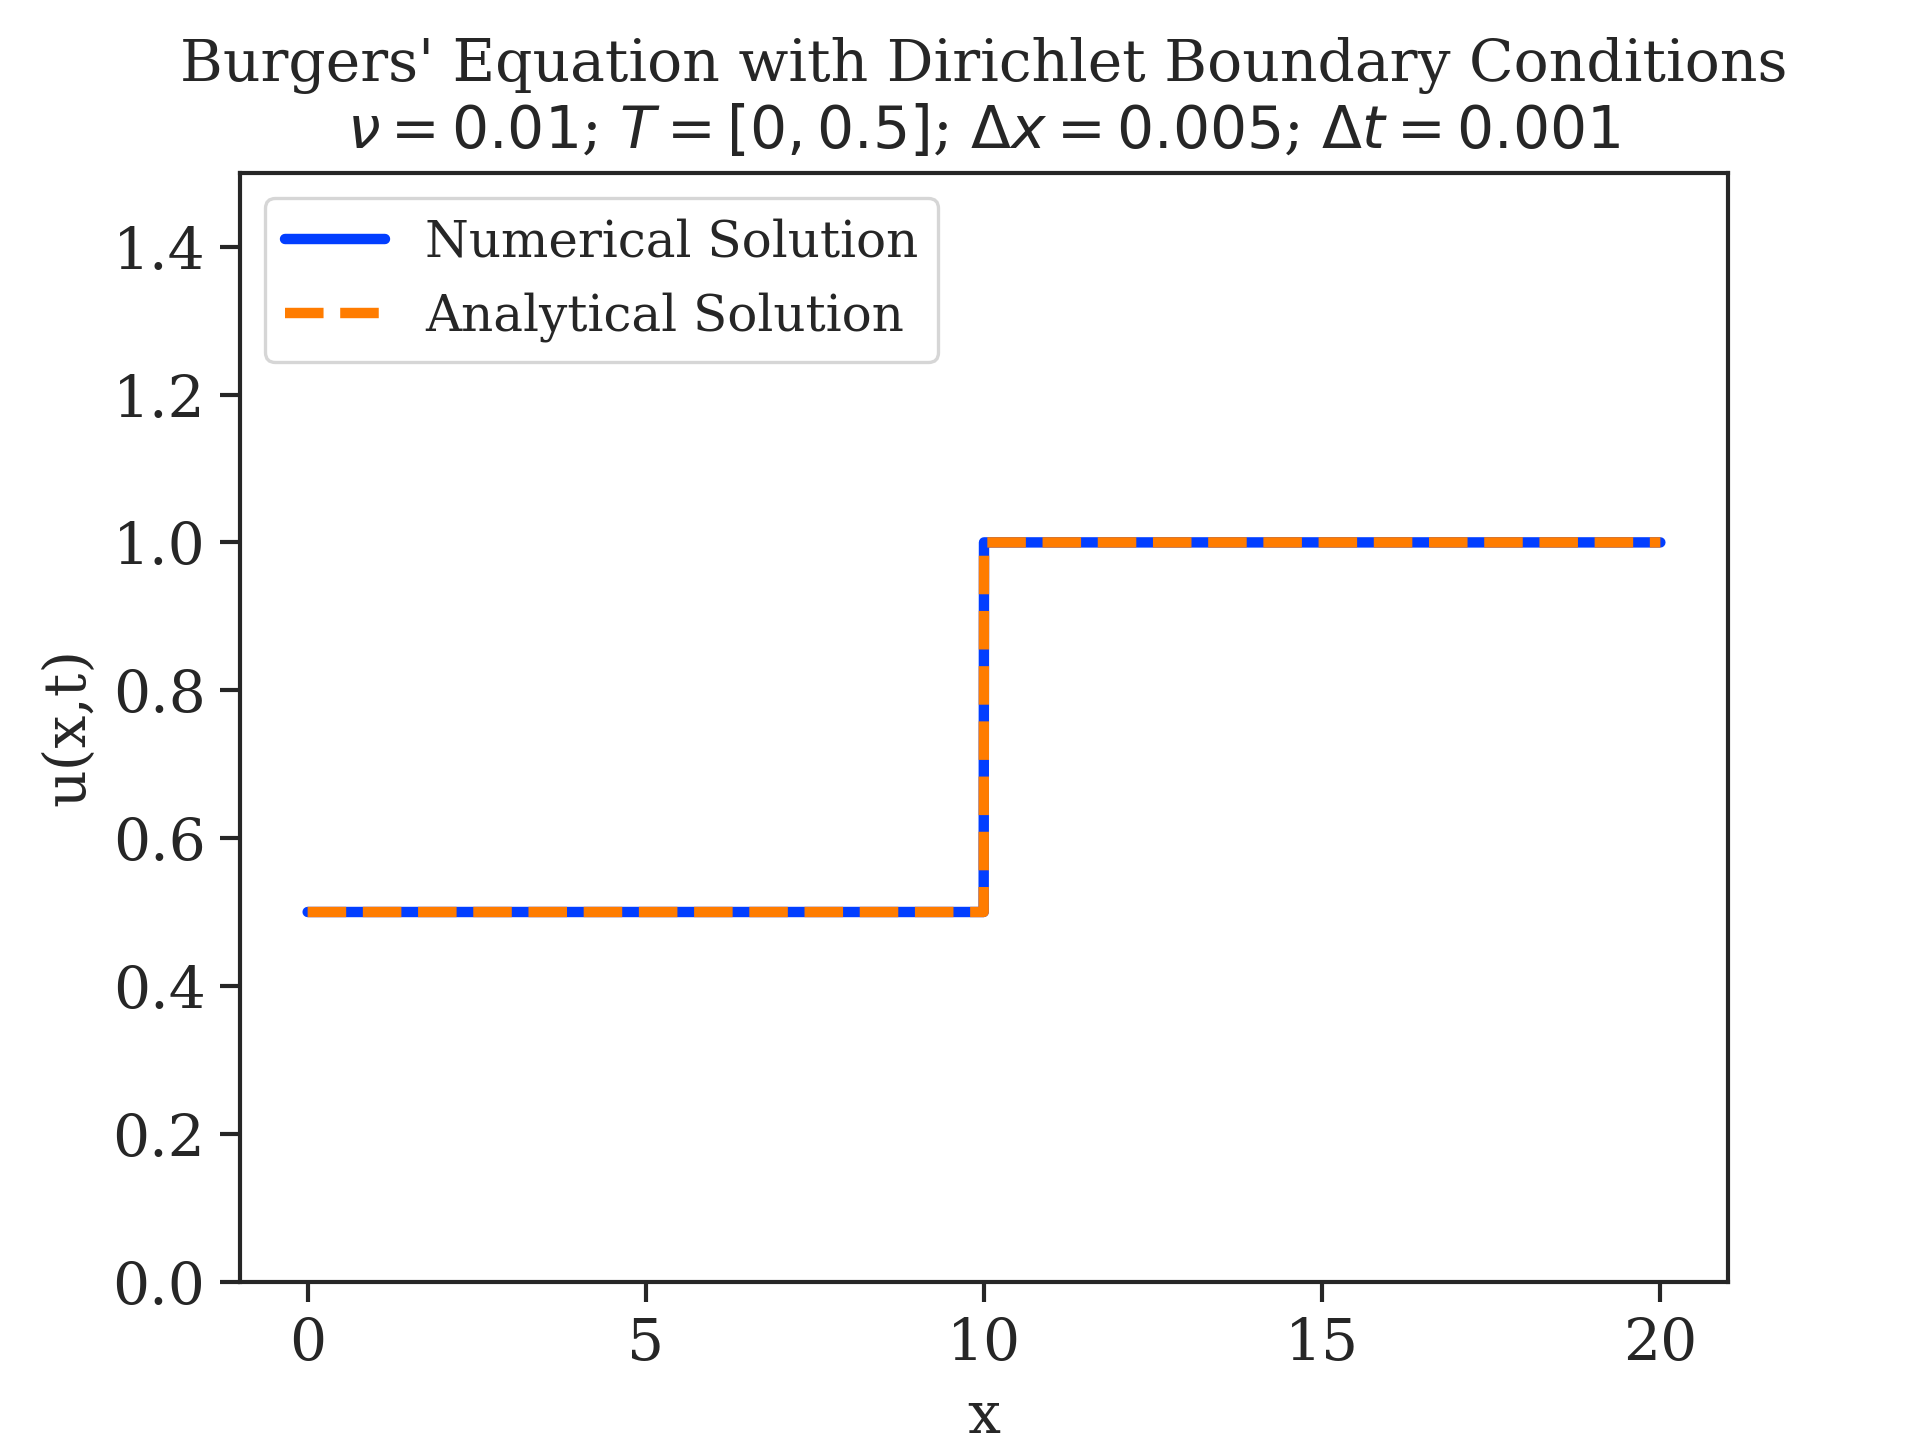
\includegraphics[width=0.8\textwidth]{../dirichlet_BC/images_nu=0.01/0_plot}
	\caption{Implemented initial condition.}
	\label{fig:initial condition}
\end{figure}

\begin{figure}
	\centering
	\begin{subfigure}{0.55\linewidth}
		\centering
		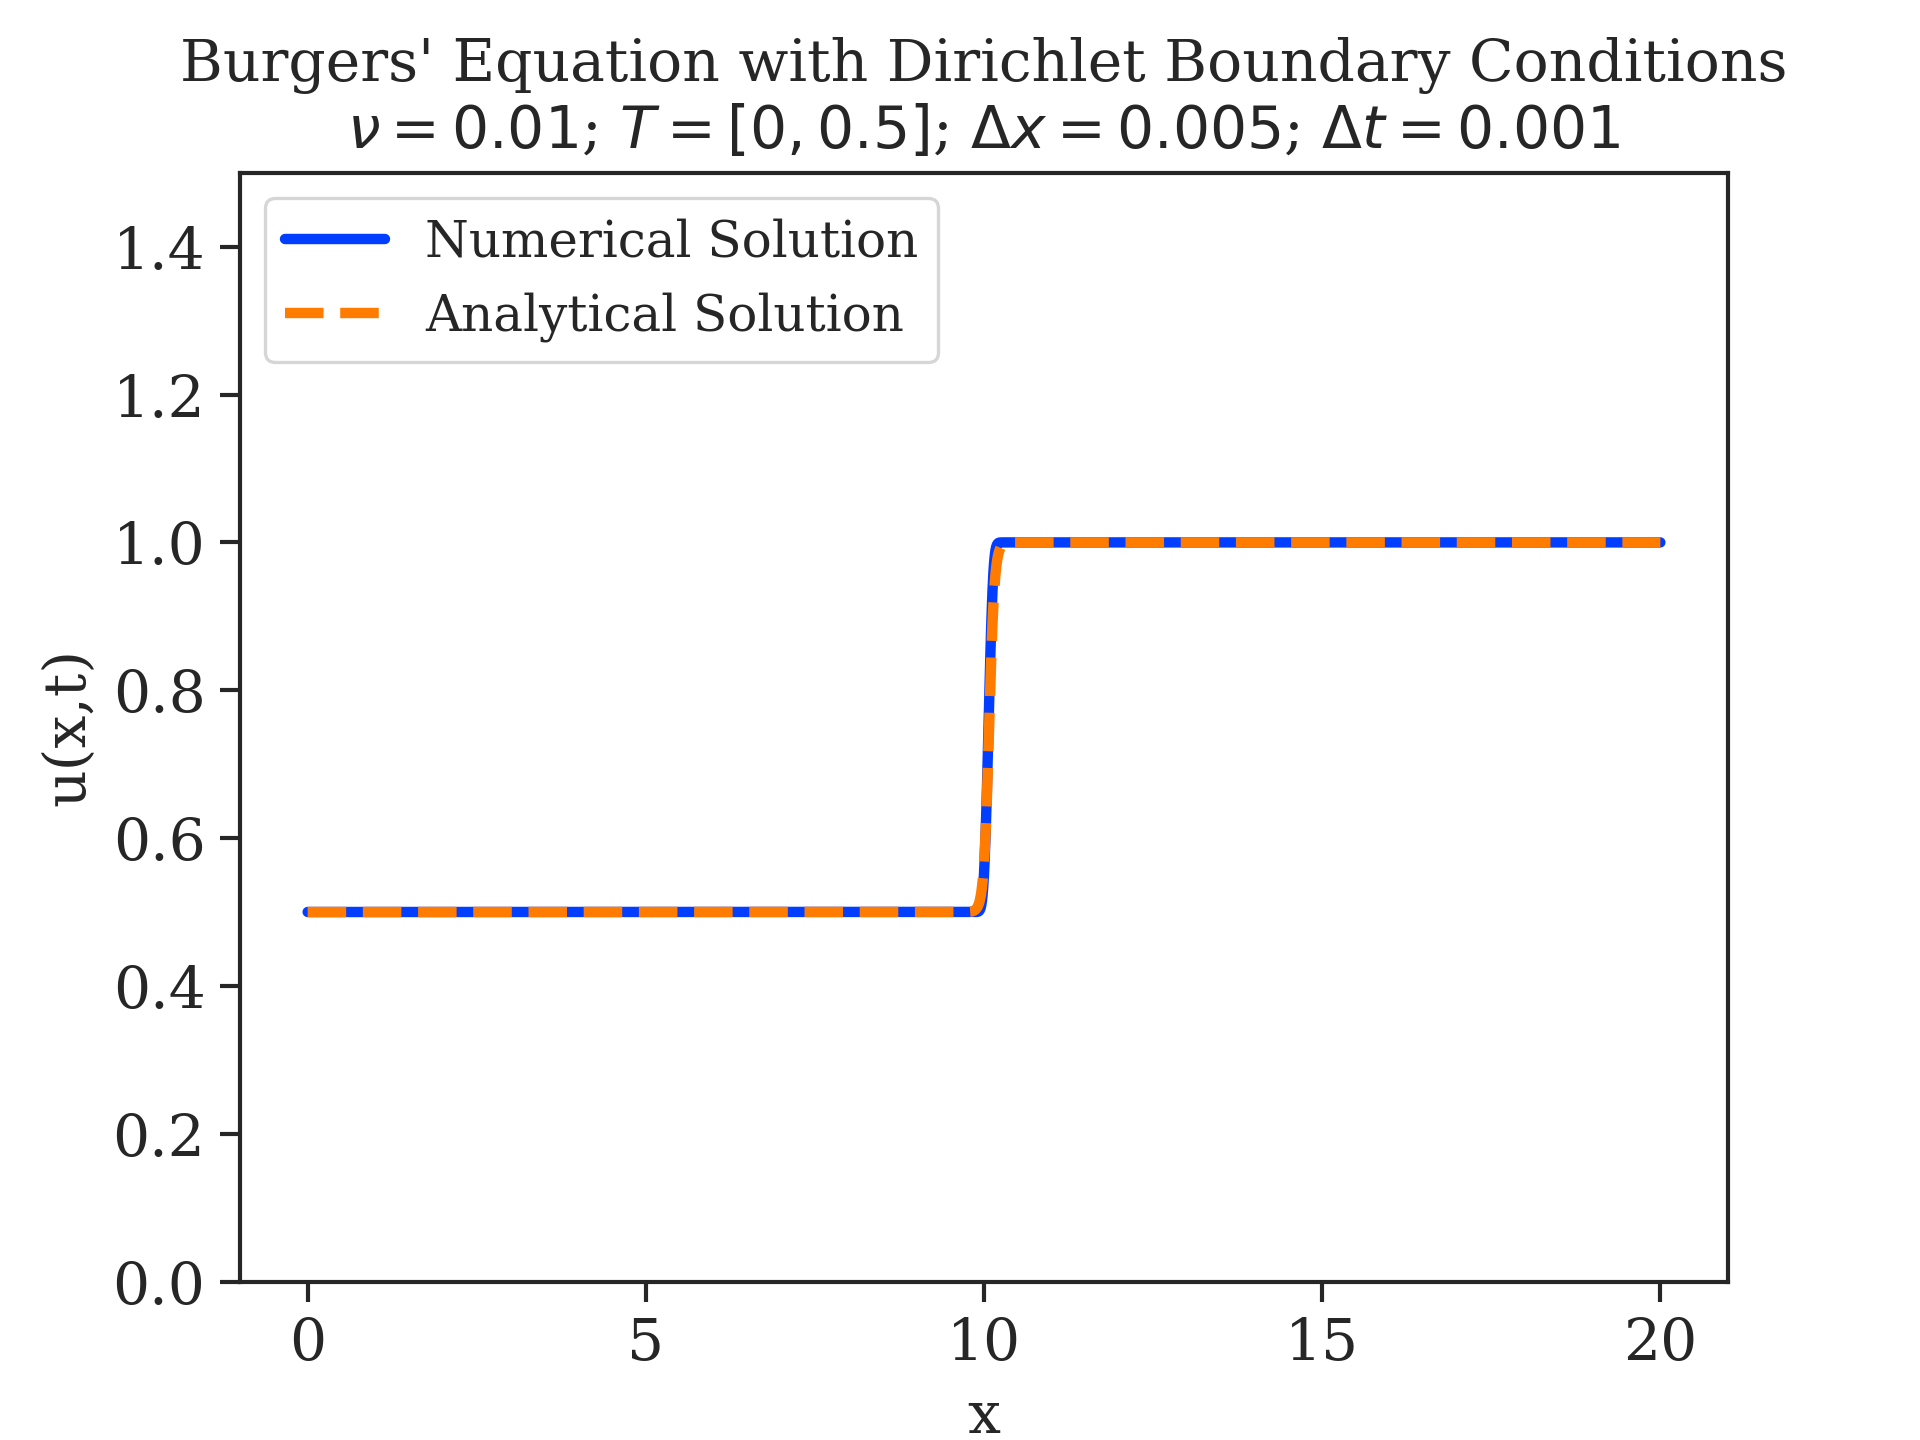
\includegraphics[width=\linewidth]{../dirichlet_BC/images_nu=0.01/100_plot}
		\caption{Inhomogeneous Dirichlet}
	\end{subfigure}
	\hfill
	\begin{subfigure}{0.55\linewidth}
		\centering
		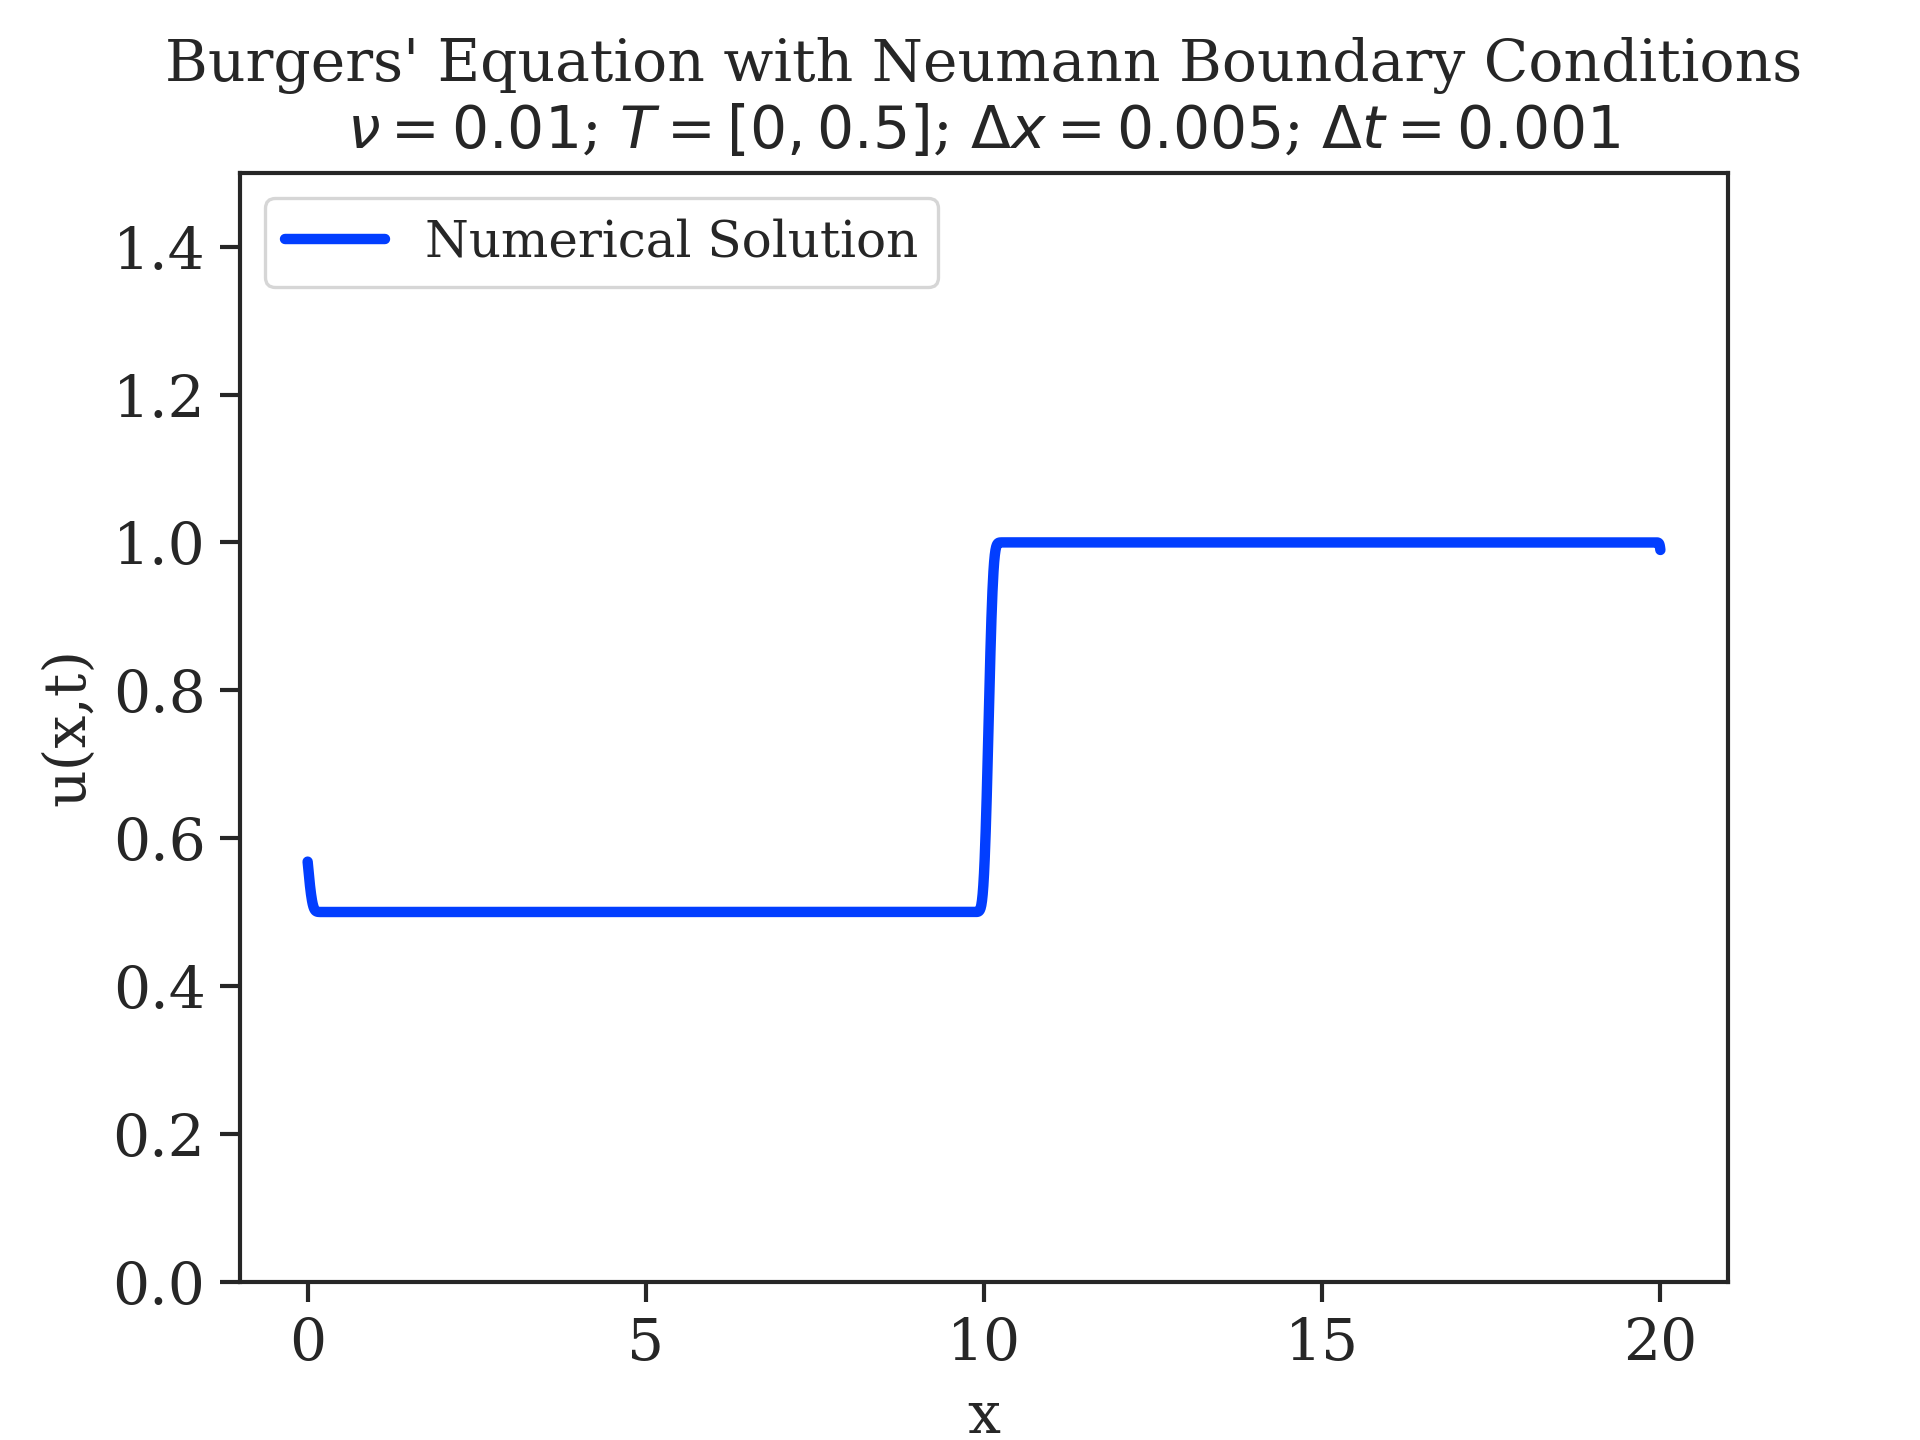
\includegraphics[width=\linewidth]{../neumann_BC/images_nu=0.01/100_plot}
		\caption{Inhomogeneous Neumann}
	\end{subfigure}
	\hfill
	\begin{subfigure}{0.55\linewidth}
		\centering
		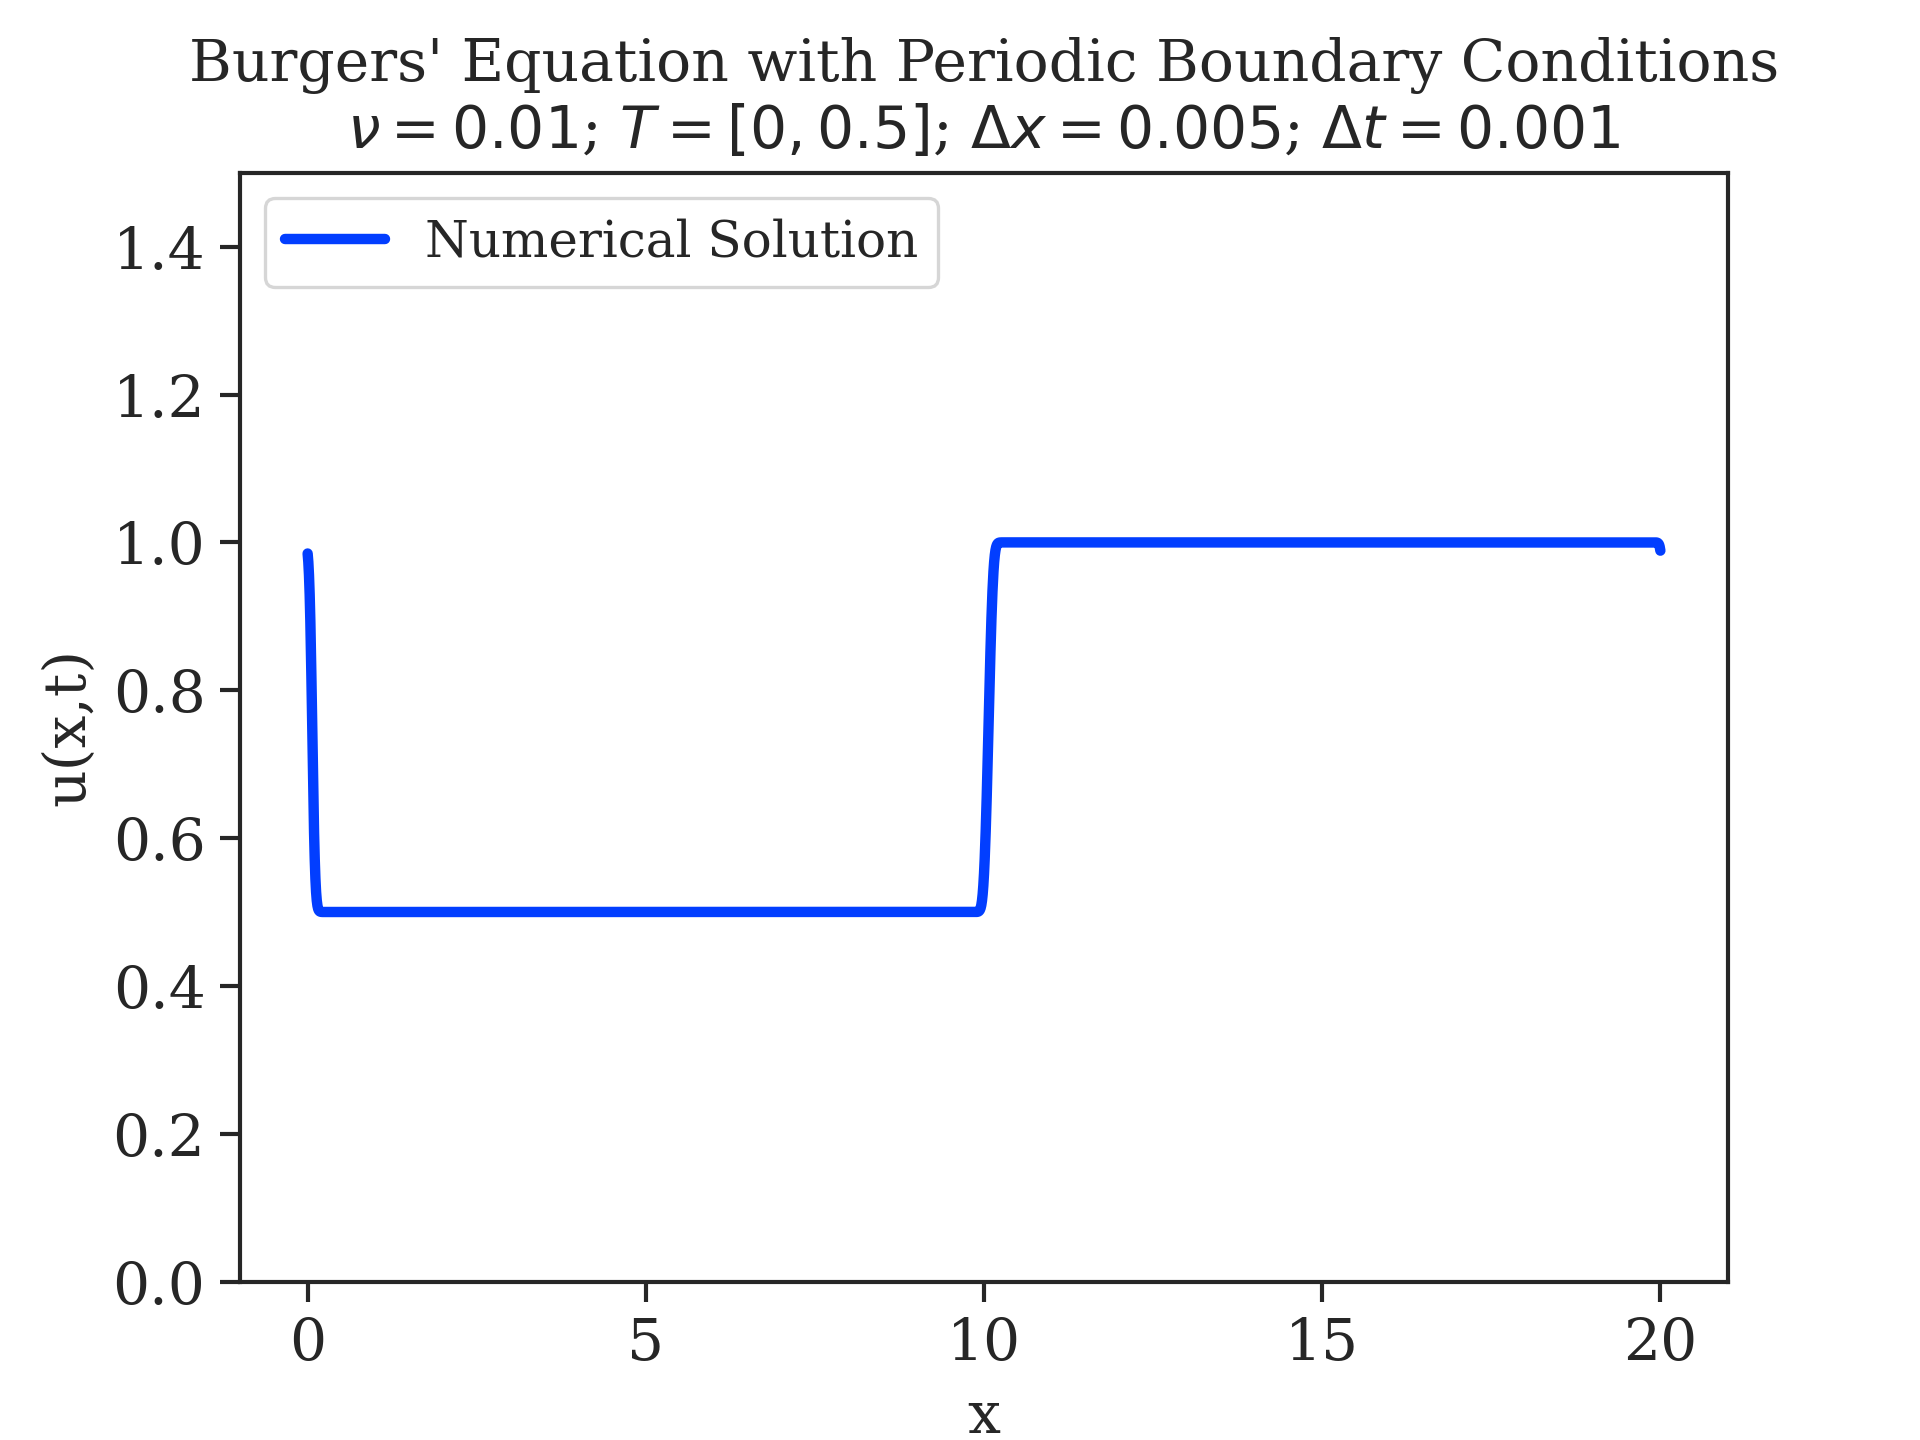
\includegraphics[width=\linewidth]{../periodic_BC/images_nu=0.01/100_plot}
		\caption{Periodic}
	\end{subfigure}

	\caption{Implemented conditions $t=0.10$.}
	\label{fig:0.1-figures}
\end{figure}

\begin{figure}
	\centering
	\begin{subfigure}{0.55\linewidth}
		\centering
		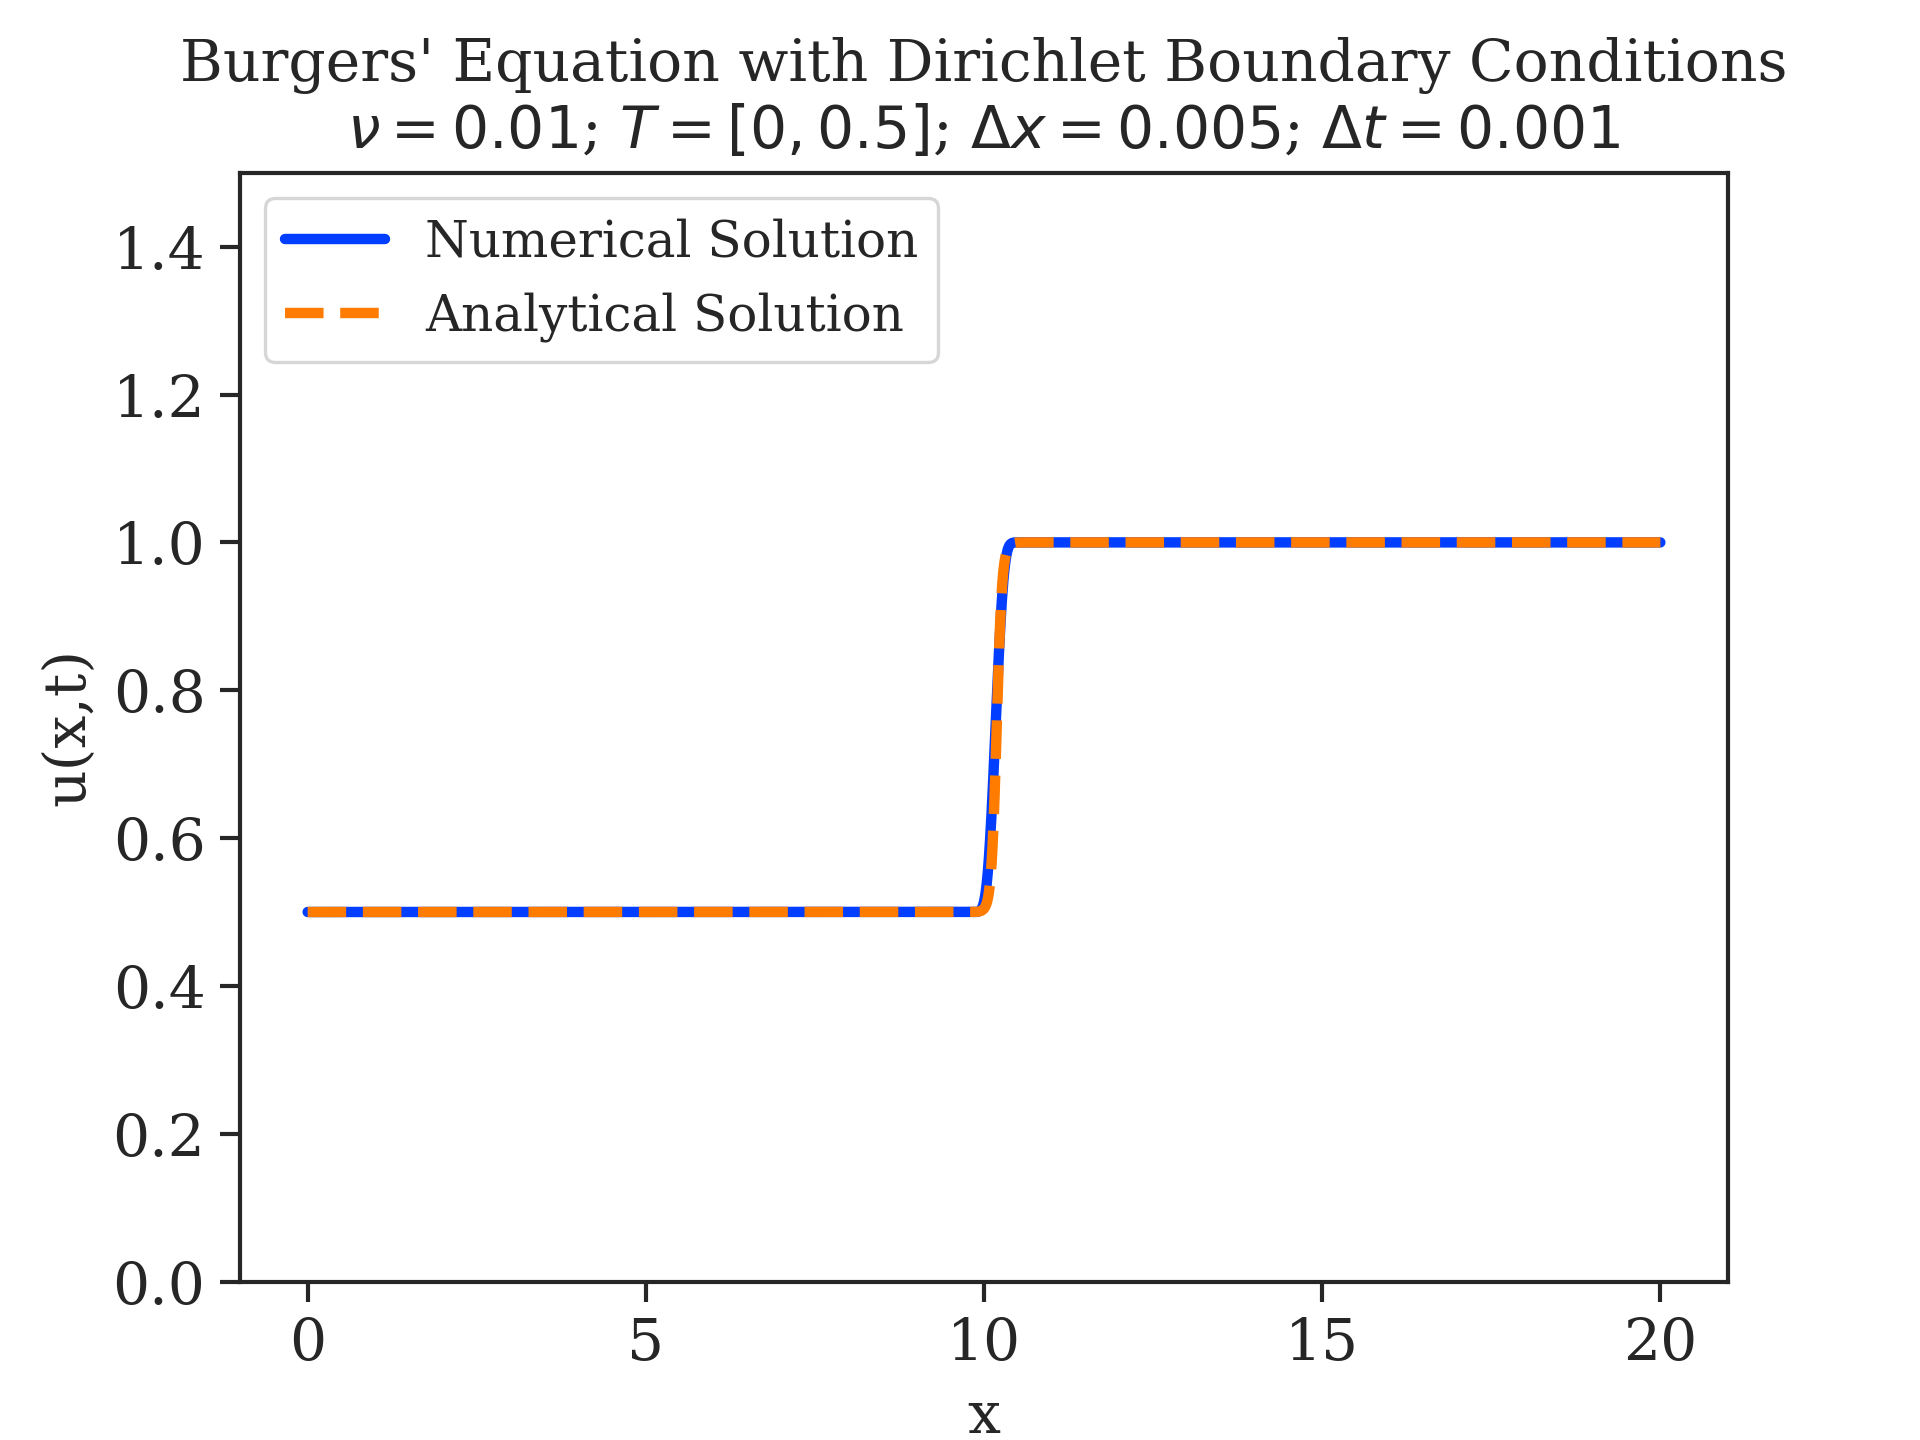
\includegraphics[width=\linewidth]{../dirichlet_BC/images_nu=0.01/250_plot}
		\caption{Inhomogeneous Dirichlet}
	\end{subfigure}
	\hfill
	\begin{subfigure}{0.55\linewidth}
		\centering
		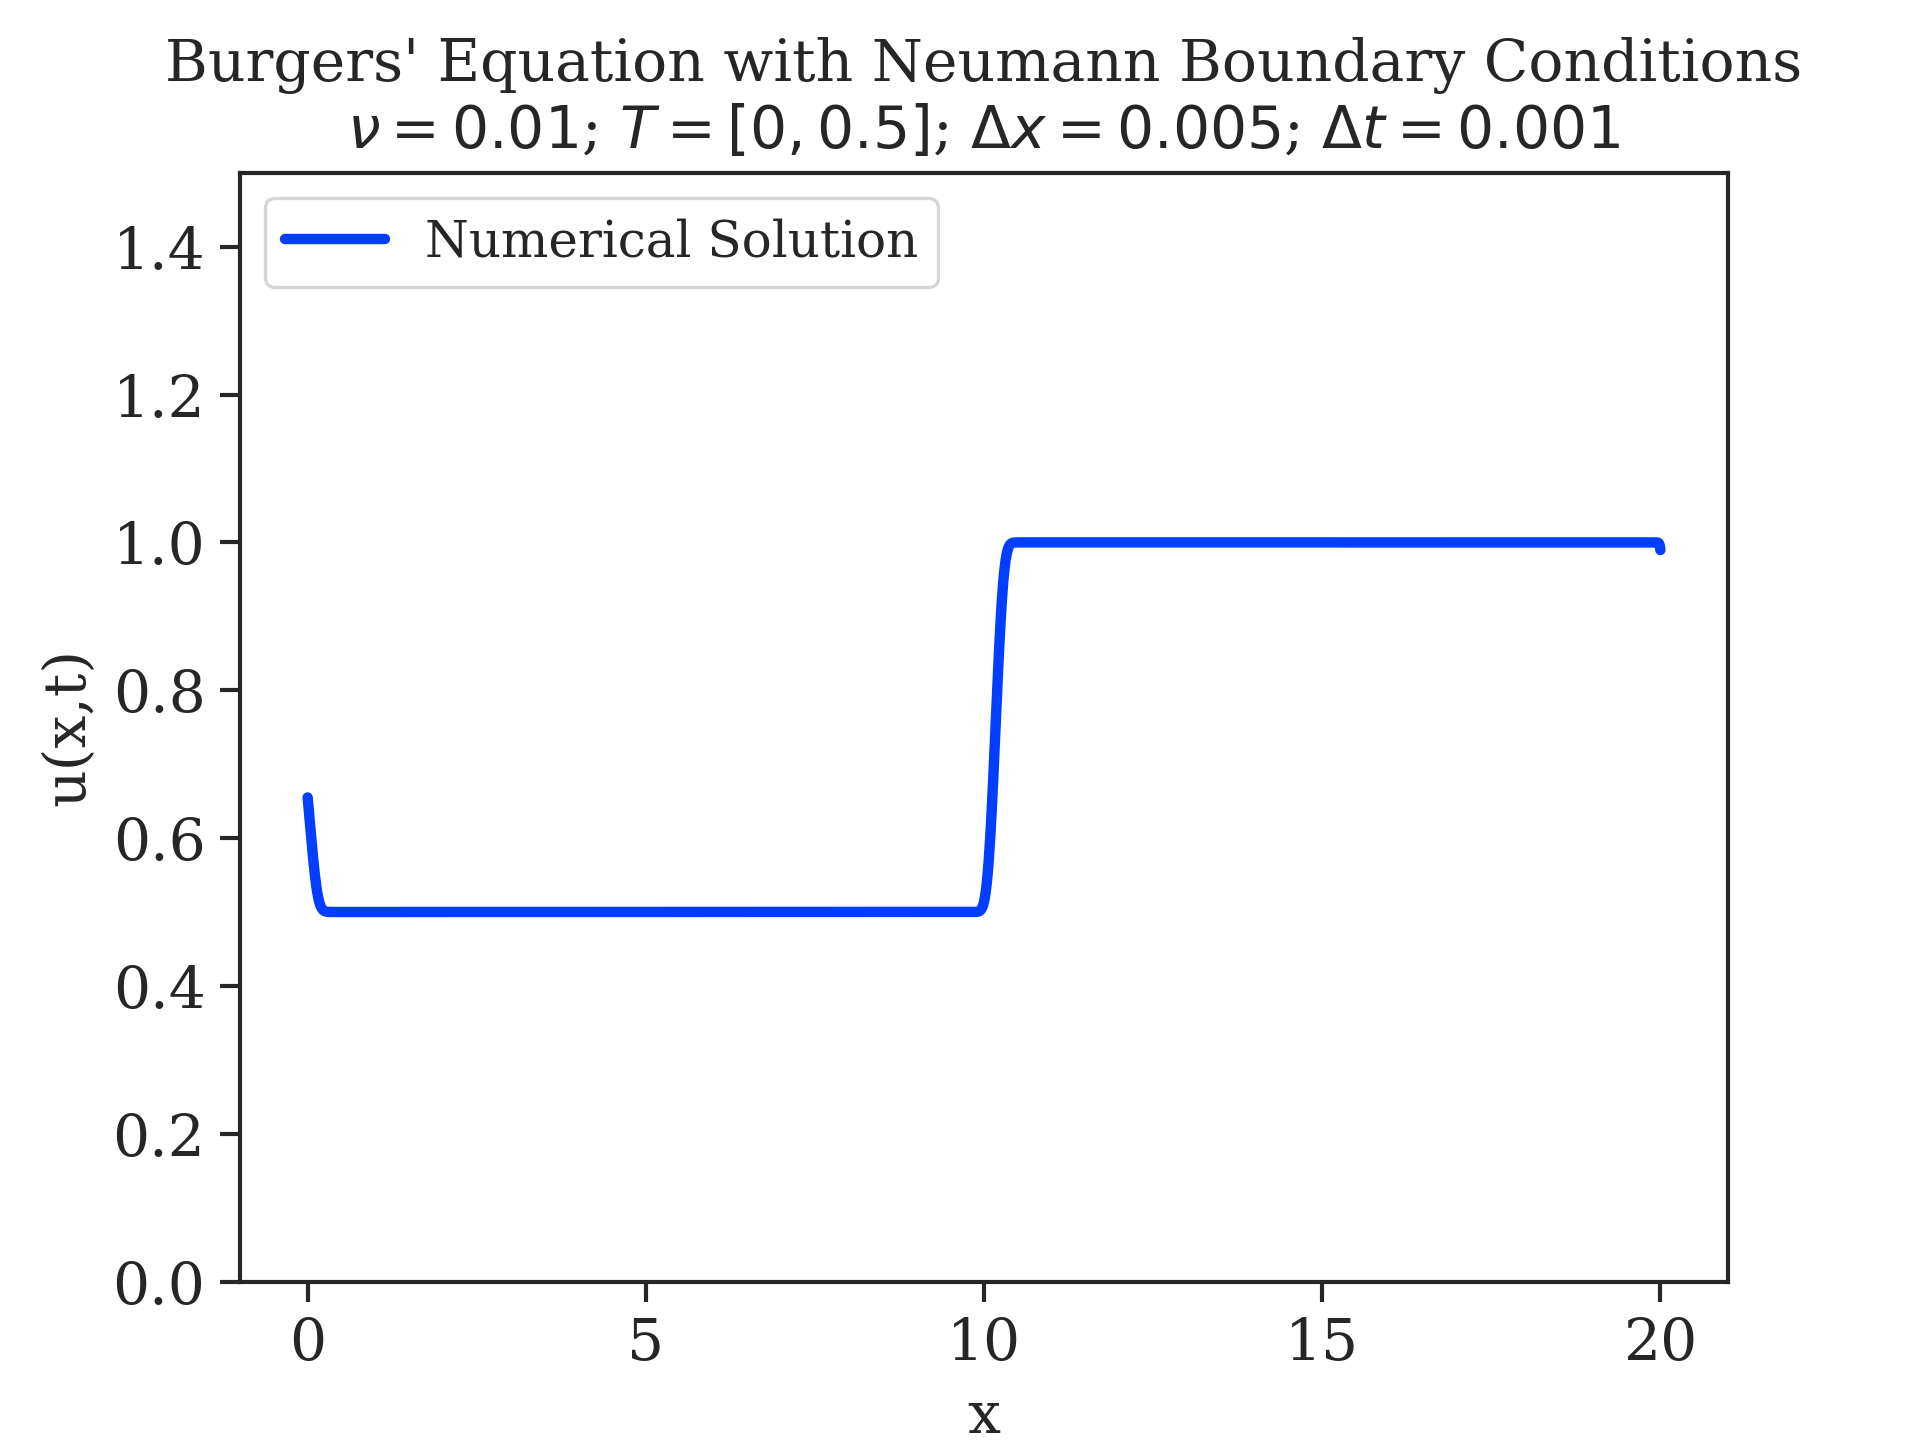
\includegraphics[width=\linewidth]{../neumann_BC/images_nu=0.01/250_plot}
		\caption{Inhomogeneous Neumann}
	\end{subfigure}
	\hfill
	\begin{subfigure}{0.55\linewidth}
		\centering
		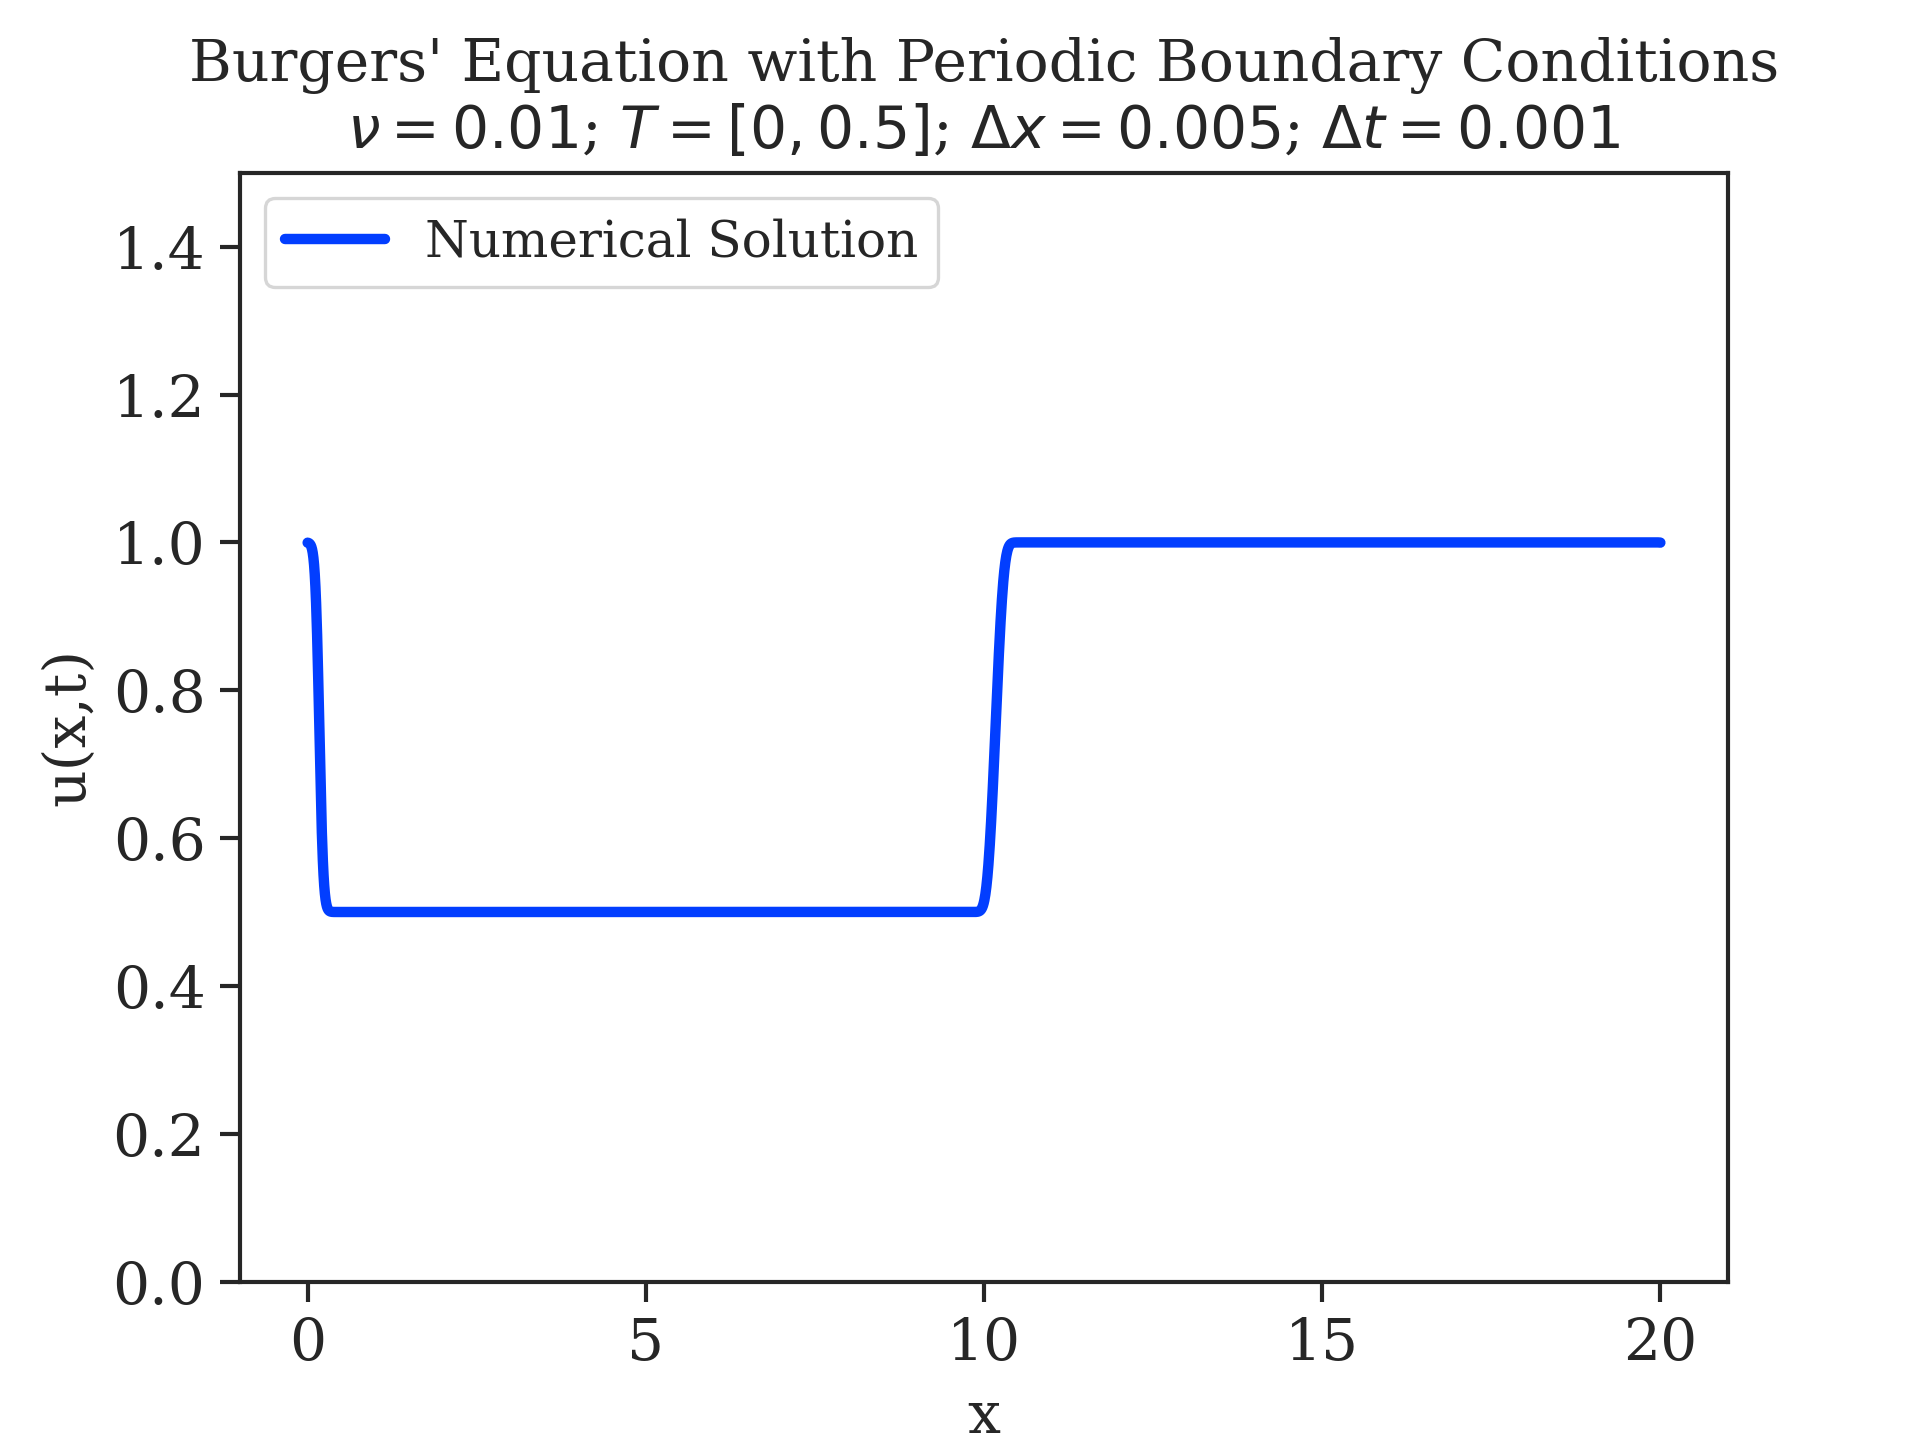
\includegraphics[width=\linewidth]{../periodic_BC/images_nu=0.01/250_plot}
		\caption{Periodic}
	\end{subfigure}

	\caption{Implemented conditions $t=0.25$.}
	\label{fig:0.25-figures}
\end{figure}

\begin{figure}
	\centering
	\begin{subfigure}{0.55\linewidth}
		\centering
		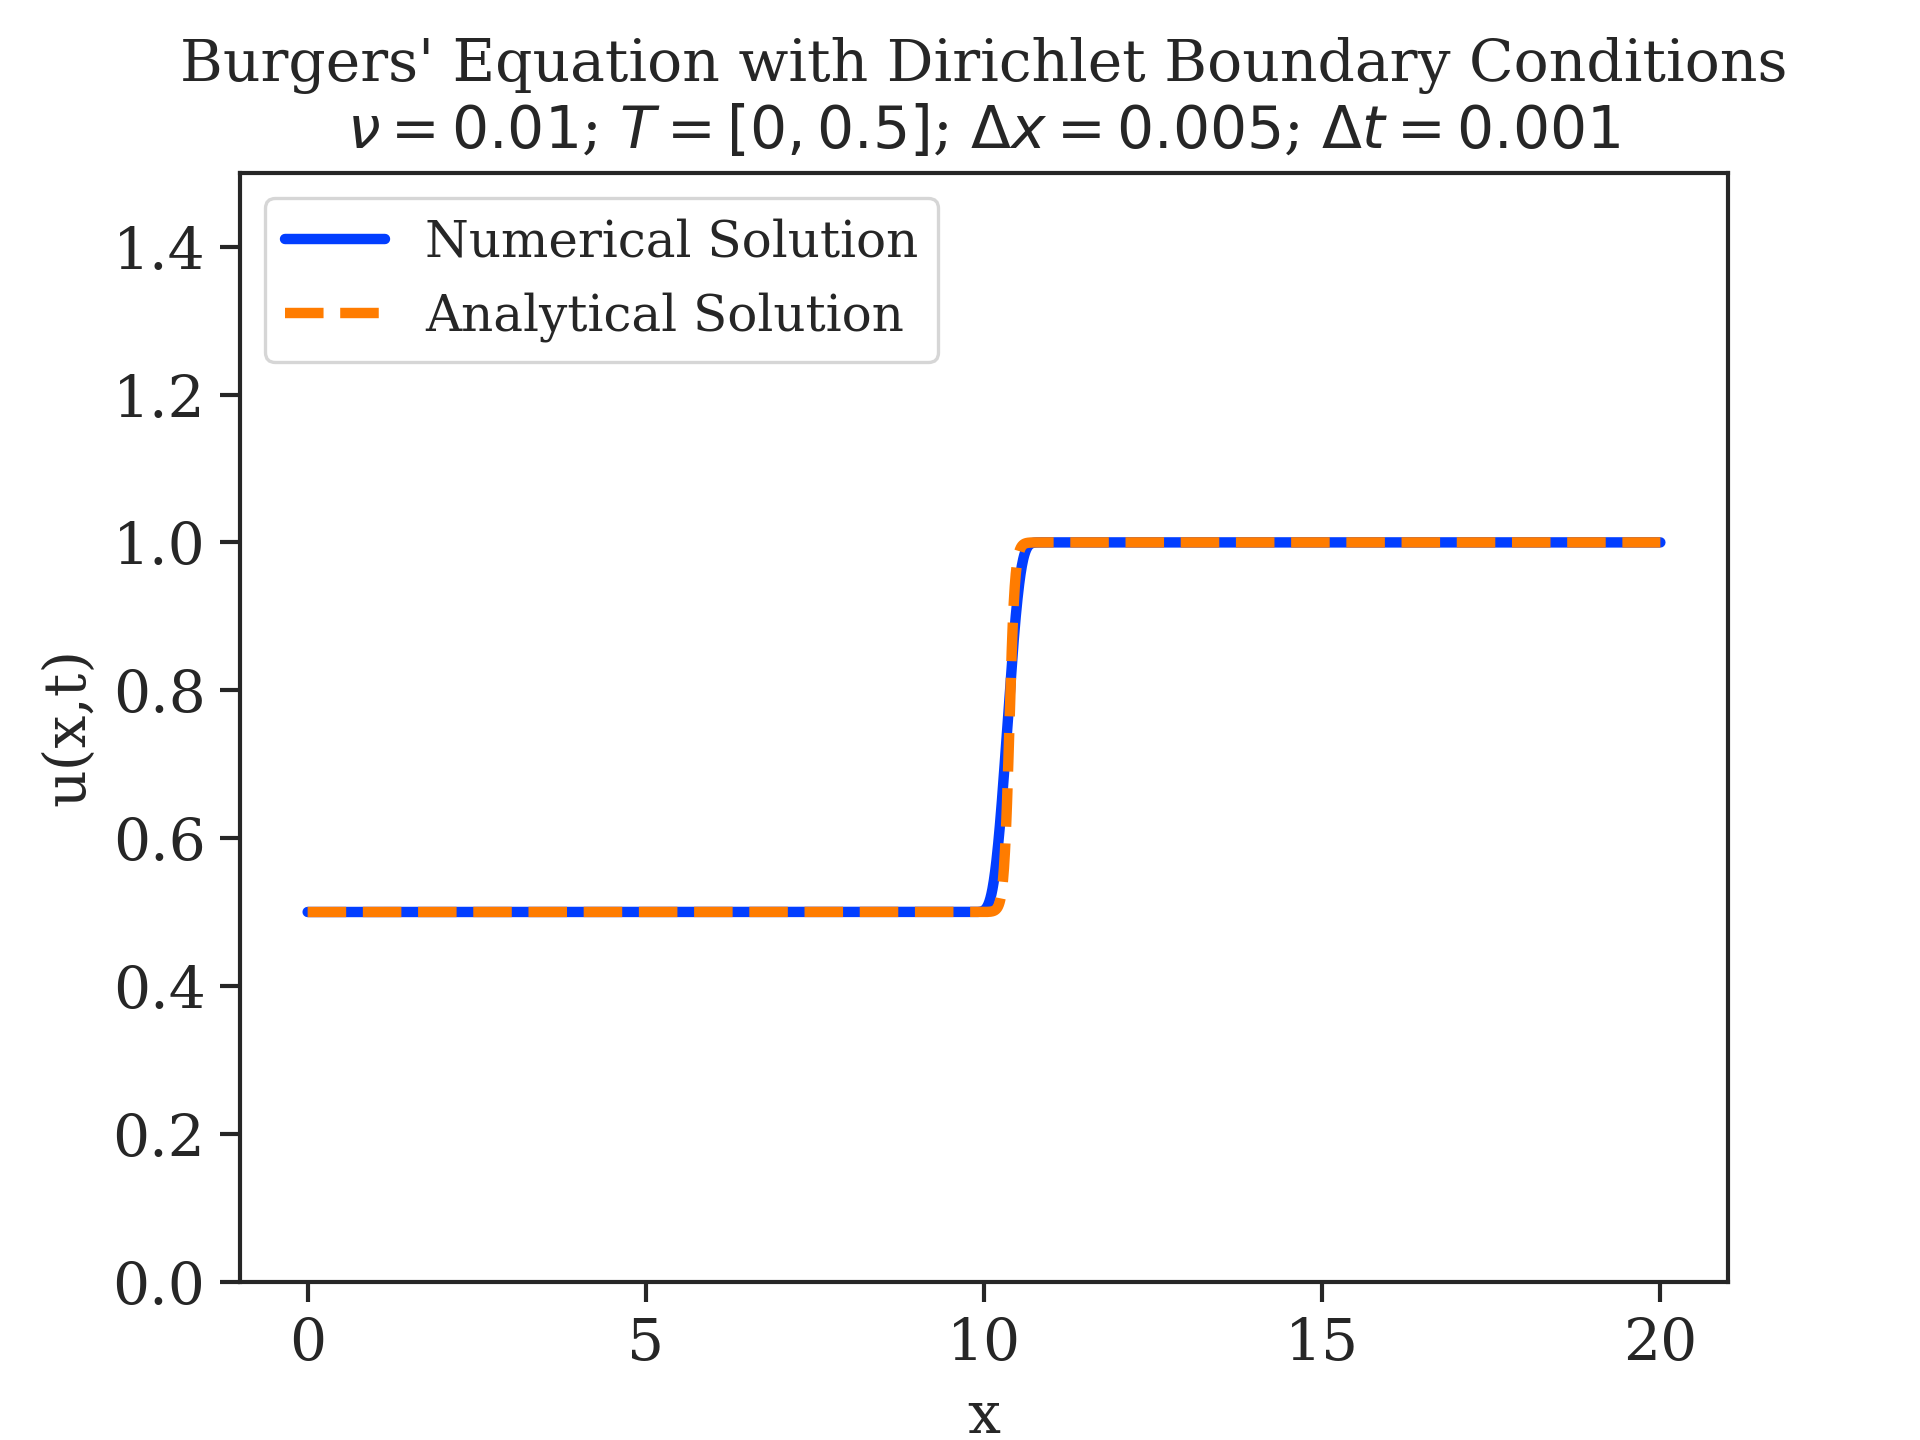
\includegraphics[width=\linewidth]{../dirichlet_BC/images_nu=0.01/500_plot}
		\caption{Inhomogeneous Dirichlet}
	\end{subfigure}
	\hfill
	\begin{subfigure}{0.55\linewidth}
		\centering
		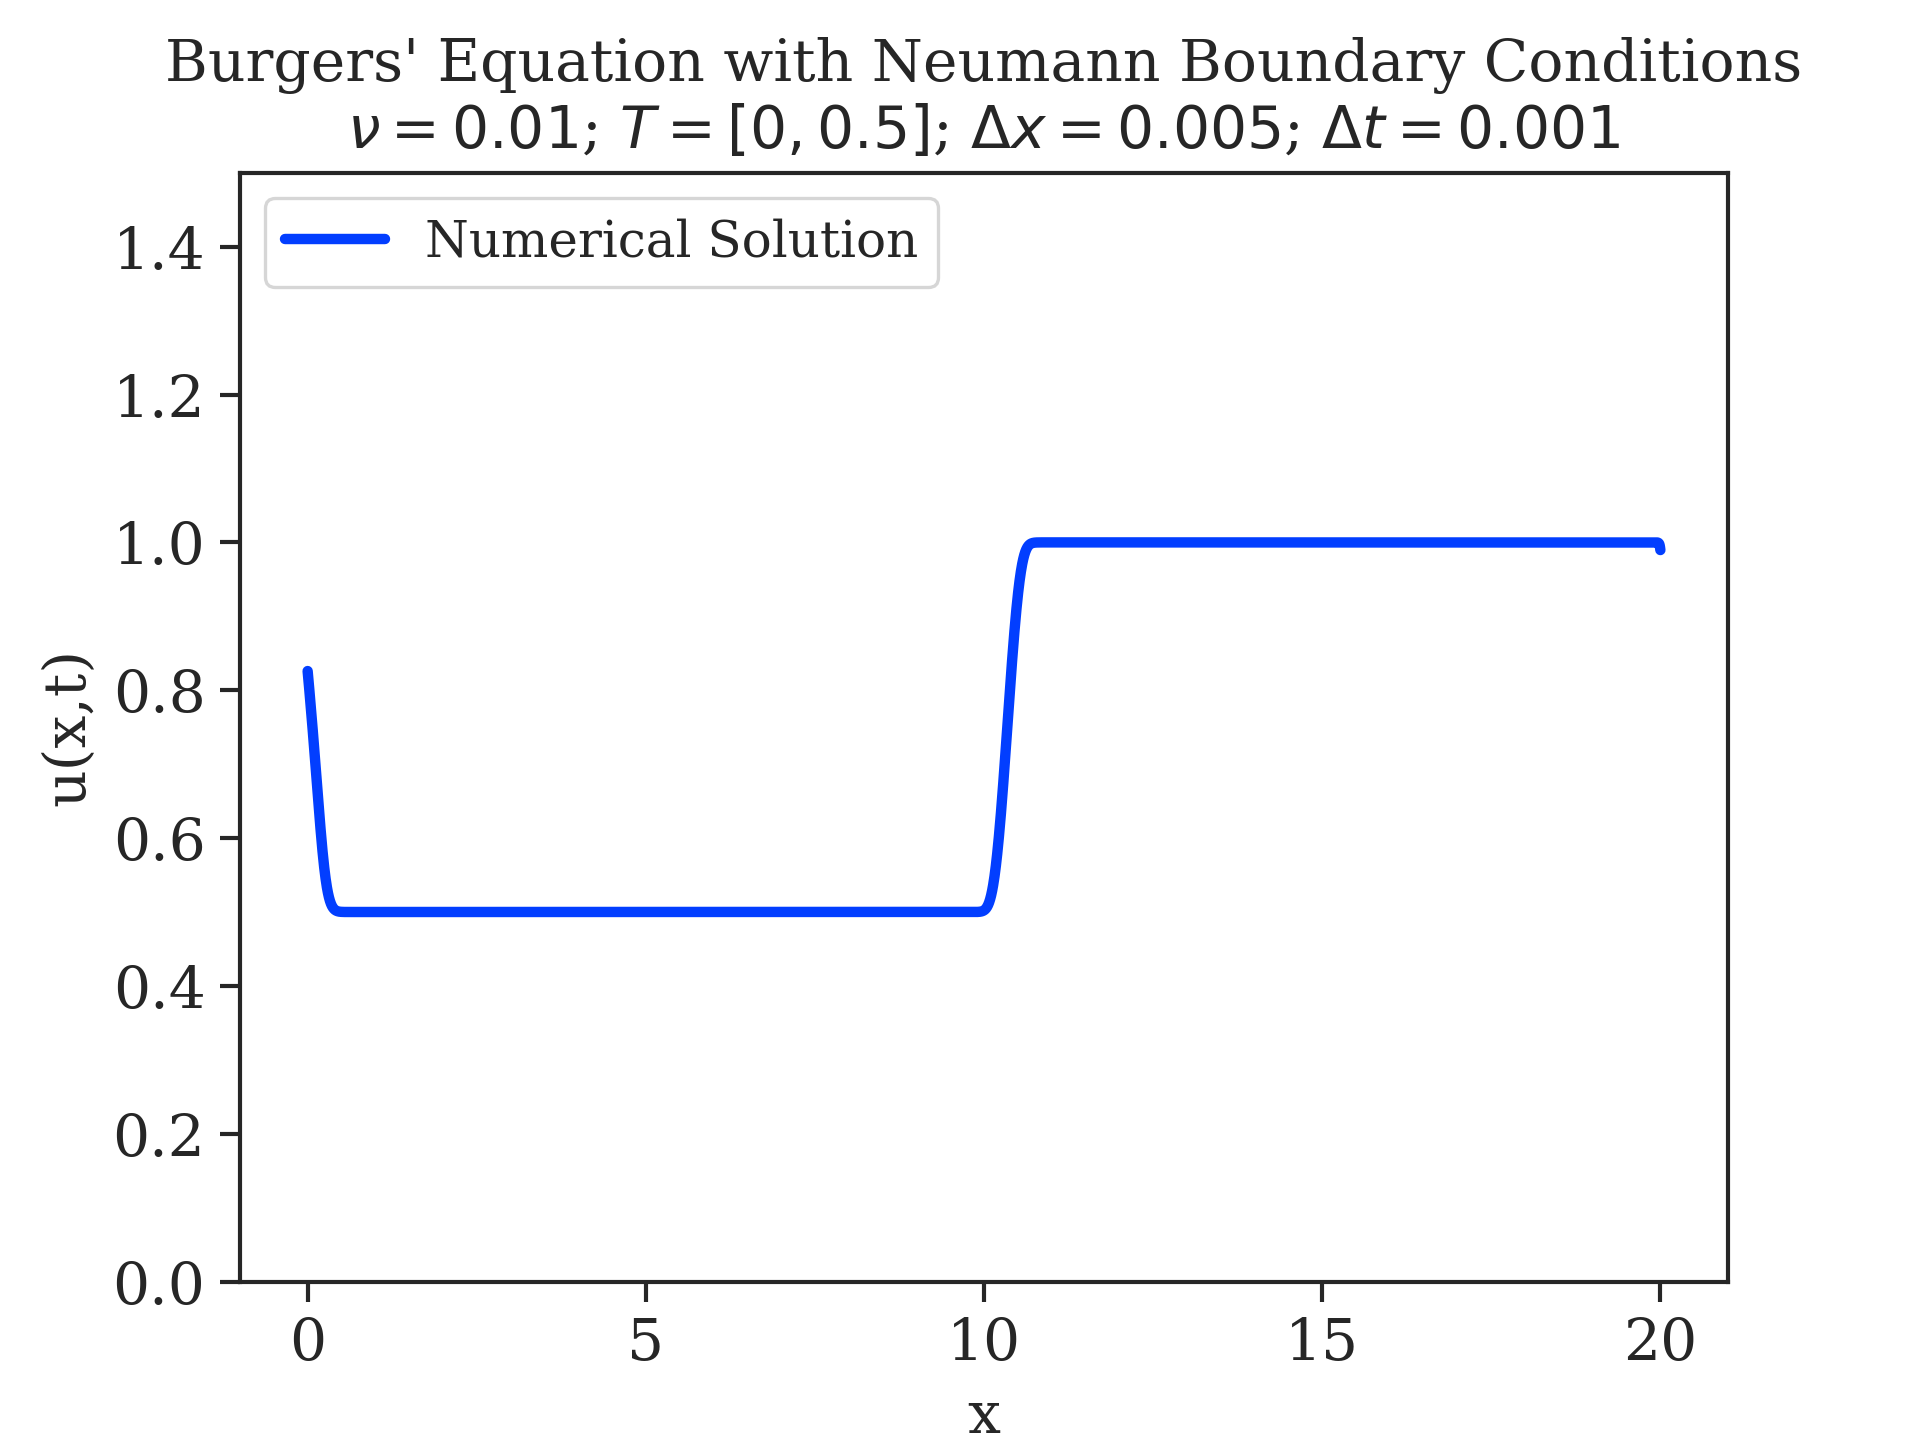
\includegraphics[width=\linewidth]{../neumann_BC/images_nu=0.01/500_plot}
		\caption{Inhomogeneous Neumann}
	\end{subfigure}
	\hfill
	\begin{subfigure}{0.55\linewidth}
		\centering
		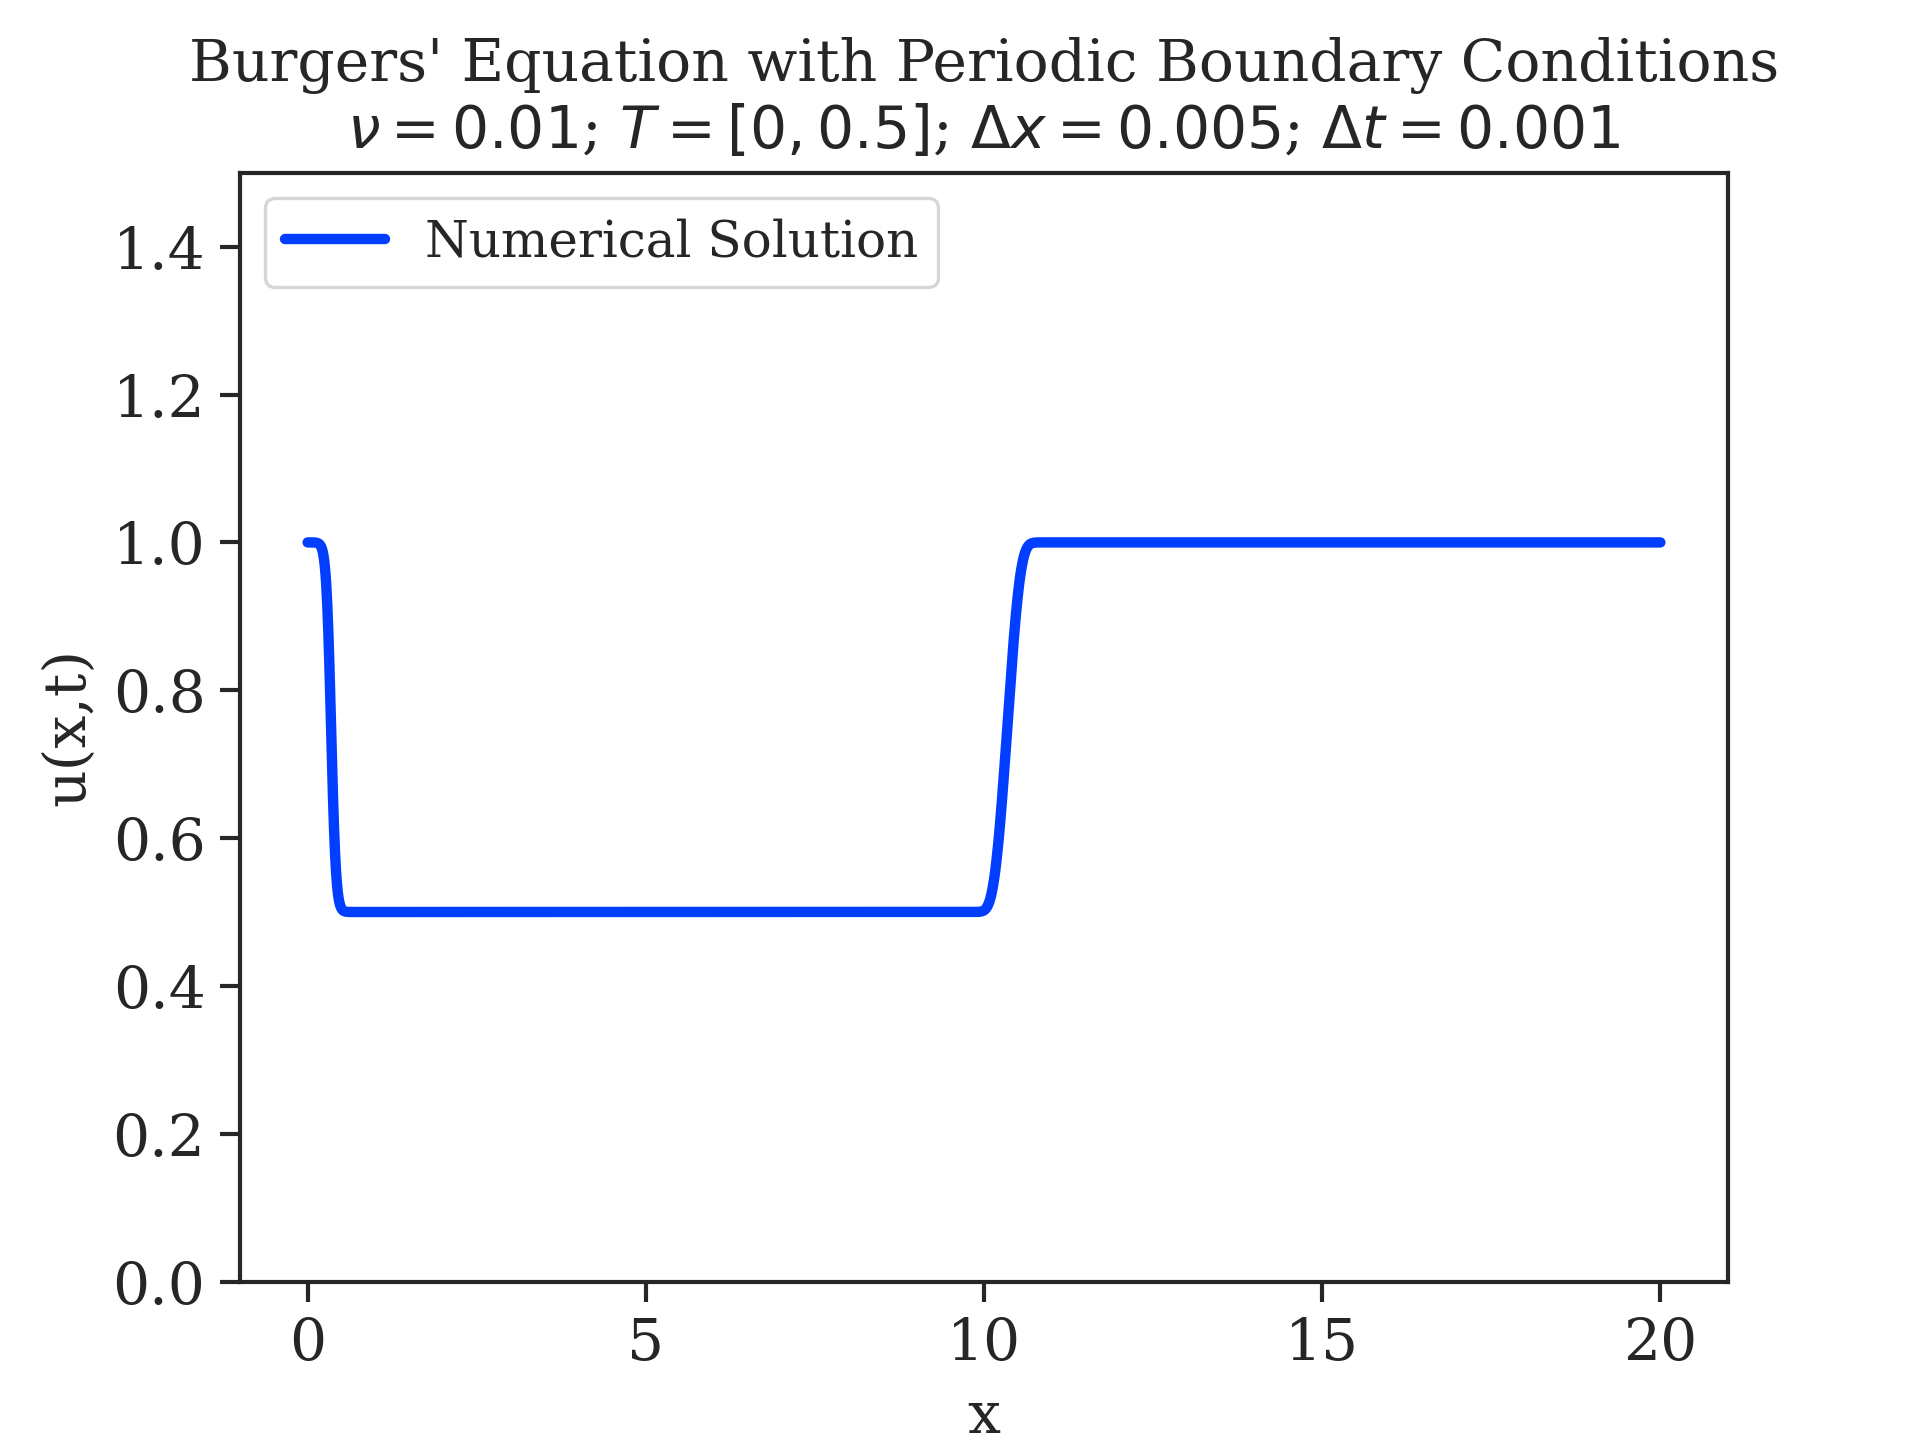
\includegraphics[width=\linewidth]{../periodic_BC/images_nu=0.01/500_plot}
		\caption{Periodic}
	\end{subfigure}
	\hfill

	\caption{Implemented conditions $t=0.50$.}
	\label{fig:final-figures}
\end{figure}

As mentioned in \cref{sec:problem-statement}, Burgers' equation was developed to study shocks and rarefactions in fluids, which that occur due to the nonlinear advective term present in the Navier-Stokes equations.
Because this paper's focus was on numerical methods and implementation, a mathematical analysis of these phenomena are not included.
For more studies on shocks and Burgers' equation, the author recommends~\autocite{salihBurgersEquation2016,cameronNOTESBURGERSEQUATION} among other resources.
	\clearpage


	\section{Conclusion and Next Steps}\label{sec:conclusion}
	For any who have been able to run the included code above $\nu=0.01$, you will notice that the solution rapidly diverges at the interface of the two velocities in the initial condition.
	Though it is not immediately clear what the cause of this instability is, the next steps will likely include explorations of higher-resolution spatial and flux schemes.
	A finer mesh may also greatly improve the quality of the solution, though this will be difficult to achieve without the aid of parallel computing to handle the large matrix-vector products.
	Finally, a conversion from an explicit time-stepping method (RK4) to an implicit method may also improve stability properties.
	As can be shown in the literature~\autocite{cameronNOTESBURGERSEQUATION,salihBurgersEquation2016}, the discontinuity present in the solution is a known computational difficulty, and its study will help greatly in understanding more complex equations such as the Navier-Stokes, which also have nonlinearities.


%%%%%%%%%%%%%%%%%%%%%%%%%%%%%%%%%%%%%%%%%%%%%%%%%%%%%%%%%%%%%%%%%%%%%%%%%%%%%%%
% REFERENCES
%%%%%%%%%%%%%%%%%%%%%%%%%%%%%%%%%%%%%%%%%%%%%%%%%%%%%%%%%%%%%%%%%%%%%%%%%%%%%%%

% Bibliography support via biblatex


	\section{REFERENCES}% Create heading for references to include in ToC.
	\printbibliography[heading=none]% Print references without biblatex's heading.

%%%%%%%%%%%%%%%%%%%%%%%%%%%%%%%%%%%%%%%%%%%%%%%%%%%%%%%%%%%%%%%%%%%%%%%%%%%%%%%
% APPENDICES
%%%%%%%%%%%%%%%%%%%%%%%%%%%%%%%%%%%%%%%%%%%%%%%%%%%%%%%%%%%%%%%%%%%%%%%%%%%%%%%
	\appendix
	\acresetall % Reset abbreviations for Appendices.


	\section{Splitting a Matrix-Vector Multiply} \label{sec:matrix-vector-multiply}
	Say we have a system $A\mathbf{x}=\mathbf{b}$, and we simply want to evaluate the left-hand-side to verify the result.
	If $A$ is $3\times 3$ where:
	\begin{equation}
		\label{eq:a-matrix}
		A = \begin{bmatrix}
				a & b & c \\
				d & e & f \\
				g & h & i \\
		\end{bmatrix}
	\end{equation}
	and:
	\begin{equation}
		\label{eq:x_vec}
		\mathbf{x} =
		\begin{bmatrix}
			x_1 \\
			x_2 \\
			x_3
		\end{bmatrix},
	\end{equation}
	then their product is:
	\begin{equation}
		\label{eq:ax-product}
		\begin{bmatrix}
			a & b & c \\
			d & e & f \\
			g & h & i \\
		\end{bmatrix}
		\begin{bmatrix}
			x_1 \\
			x_2 \\
			x_3
		\end{bmatrix}=
		\begin{bmatrix}
			ax_1+bx_2+cx_3 \\
			dx_1+ex_2+fx_3 \\
			gx_1+hx_2+ix_3
		\end{bmatrix}
	\end{equation}
	which can also be expressed as:
	\begin{equation}
		\label{eq:matrix-expansion}
		\begin{split}
			\begin{bmatrix}
				ax_1+bx_2+cx_3 \\
				dx_1+ex_2+fx_3 \\
				gx_1+hx_2+ix_3
			\end{bmatrix}
			&=
			\begin{bmatrix}
				ax_1 \\
				bx_1 \\
				cx_1
			\end{bmatrix}+\begin{bmatrix}
							  bx_2+cx_3 \\
							  ex_2+fx_3 \\
							  hx_2+ix_3
			\end{bmatrix}\\
			&=
			\begin{bmatrix}
				a \\
				b \\
				c
			\end{bmatrix}x_1 +
			\begin{bmatrix}
				b & c \\
				e & f \\
				h & i
			\end{bmatrix}\begin{bmatrix}
							 x_2 \\
							 x_3
			\end{bmatrix}
		\end{split}.
	\end{equation}
	The above is particularly useful when a value is known, such as in the case of Dirichlet boundary conditions for a PDE.


%%%%%%%%%%%%%%%%%%%%%%%%%%%%%%%%%%%%%%%%%%%%%%%%%%%%%%%%%%%%%%%%%%%%%%%%%%%%%%%
% Back cover page
	\backmatter

%%%%%%%%%%%%%%%%%%%%%%%%%%%%%%%%%%%%%%%%%%%%%%%%%%%%%%%%%%%%%%%%%%%%%%%%%%%%%%%
\end{document}
%%%%%%%%%%%%%%%%%%%%%%%%%%%%%%%%%%%%%%%%%%%%%%%%%%%%%%%%%%%%%%%%%%%%%%%%%%%%%%%
% end of ornltm/ornl-template-example.tex
%%%%%%%%%%%%%%%%%%%%%%%%%%%%%%%%%%%%%%%%%%%%%%%%%%%%%%%%%%%%%%%%%%%%%%%%%%%%%%%
